% SPDX-License-Identifier: GPL-3.0-or-later
\chapter{Centuri Cosmice, Planete Pitice și Asteroizi}
\label{chap:corpuri-sistem-solar}

Dincolo de cele 8 planete majore și sateliții lor naturali prezentați în Capitolul~\ref{chap:planete}, Sistemul Solar adăpostește \textbf{două centuri uriașe de corpuri minore} (Centura Principală de Asteroizi și Centura Kuiper), \textbf{5 planete pitice recunoscute de Uniunea Astronomică Internațională} (împreună cu satelitul binar \textbf{Charon}, asociat planetei pitice \textbf{Pluto}) și \textbf{5 asteroizi emblematici}.

\section{Centura Principală de Asteroizi și Centura Kuiper}
\label{sec:centuri}

În \textbf{Orbitar}, mii de corpuri stâncoase și înghețate sunt simulate simultan în timp real în cele două mari centuri circumsolare:


\subsection{Centura Principală de Asteroizi}
\begin{tcolorbox}[orbitardata, title={\textbf{Parametrii Regiunii Toroidale — Centura Principală de Asteroizi}}]
\begin{tabularx}{\textwidth}{@{}lX@{}}
\textbf{Rază interioară -- exterioară} & 2,15 UA -- 3,25 UA față de Soare \\
\textbf{Grosime verticală în modelul 3D} & 0,35 UA (2.200 asteroizi/corpuri randate prin \texttt{THREE.InstancedMesh}) \\
\textbf{Descriere științifică} & Regiune toroidală între orbitele planetelor Marte și Jupiter, populată de milioane de corpuri stâncoase și metalice rămase de la formarea Sistemului Solar. \\
\end{tabularx}
\end{tcolorbox}


\subsection{Centura Kuiper}
\begin{tcolorbox}[orbitardata, title={\textbf{Parametrii Regiunii Toroidale — Centura Kuiper}}]
\begin{tabularx}{\textwidth}{@{}lX@{}}
\textbf{Rază interioară -- exterioară} & 30,50 UA -- 49,00 UA față de Soare \\
\textbf{Grosime verticală în modelul 3D} & 3,20 UA (2.800 asteroizi/corpuri randate prin \texttt{THREE.InstancedMesh}) \\
\textbf{Descriere științifică} & Disc vast de corpuri înghețate situat dincolo de orbita lui Neptun, casa planetelor pitice Pluto, Haumea și Makemake. \\
\end{tabularx}
\end{tcolorbox}


\begin{tcolorbox}[orbitarjunior, title={\textbf{Mit vs. Realitate: Cum arată în realitate zborul printr-o centură de asteroizi?}}]
În filmele SF, navele spațiale trebuie să facă slalom periculos printre stânci uriașe înghesuite unele lângă altele. \textbf{În realitate}, Centura de Asteroizi și Centura Kuiper sunt atât de vaste încât distanța medie dintre doi asteroizi de dimensiuni notabile este de \textbf{sute de mii sau milioane de kilometri} (de câteva ori distanța de la Pământ la Lună!). Toate sondele trimise de NASA și ESA (precum \emph{Pioneer}, \emph{Voyager}, \emph{Galileo}, \emph{Cassini}, \emph{New Horizons} și \emph{JUICE}) au traversat centura fără să lovească absolut nimic!
\end{tcolorbox}

\begin{table}[H]
\centering
\small
\caption{Planetele pitice și asteroizii principali din Orbitar}
\resizebox{\textwidth}{!}{%
\begin{tabular}{@{}llrrrr@{}}
\toprule
\textbf{Nume} & \textbf{Categorie} & \textbf{Distanță Soare} & \textbf{Rază medie (km)} & \textbf{Perioadă orbitală} & \textbf{Temp. medie} \\
\midrule
Ceres & Planetă pitică & 2,77 UA & 473,00 & 4,61 ani & -105$^\circ$C \\
Pluto & Planetă pitică & 39,48 UA & 1188,30 & 247,94 ani & -229$^\circ$C \\
Haumea & Planetă pitică & 43,13 UA & 780,00 & 284,12 ani & -241$^\circ$C \\
Makemake & Planetă pitică & 45,43 UA & 715,00 & 306,21 ani & -243$^\circ$C \\
Eris & Planetă pitică & 67,86 UA & 1163,00 & 558,06 ani & -243$^\circ$C \\
4 Vesta & Asteroid & 2,36 UA & 262,70 & 3,63 ani & -60$^\circ$C \\
2 Pallas & Asteroid & 2,77 UA & 256,00 & 4,62 ani & -109$^\circ$C \\
16 Psyche & Asteroid & 2,92 UA & 111,00 & 4,99 ani & -100$^\circ$C \\
101955 Bennu & Asteroid & 1,13 UA & 0,24 & 1,20 ani & 4$^\circ$C \\
99942 Apophis & Asteroid & 0,92 UA & 0,18 & 0,89 ani & 17$^\circ$C \\
\bottomrule
\end{tabular}%
}
\end{table}

\clearpage
\section{Cele 5 Planete Pitice și Sistemul Binar Pluto--Charon}

\subsection{Ceres}
\label{sec:body-ceres}
\vspace{-4pt}
{\large\itshape\color{orbitarAccent} Singura planetă pitică din Centura Principală de Asteroizi}\\[4pt]


\begin{center}
\begin{tabular}{@{}m{0.44\textwidth}@{\hspace{0.03\textwidth}}m{0.51\textwidth}@{}}
\centering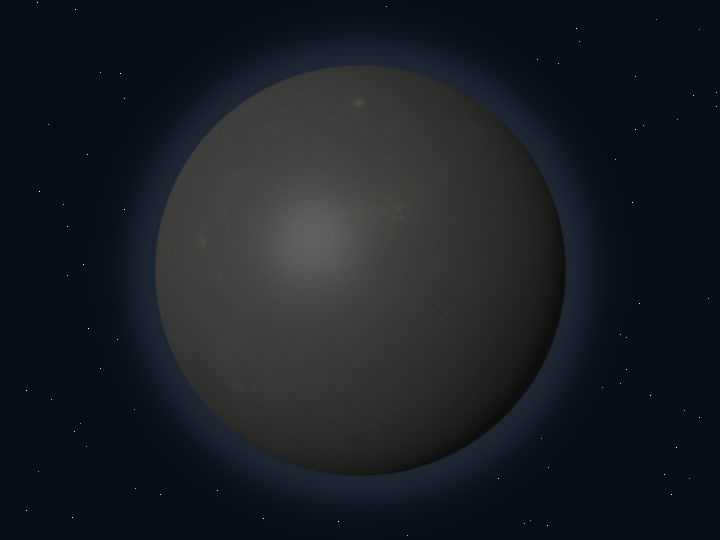
\includegraphics[width=\linewidth,height=4.4cm,keepaspectratio]{imagini/globuri/ceres.jpg}\\[2pt]
{\scriptsize\itshape\color{orbitarMuted} Vedere 3D a corpului ceresc (\textbf{Ceres})}
&
\centering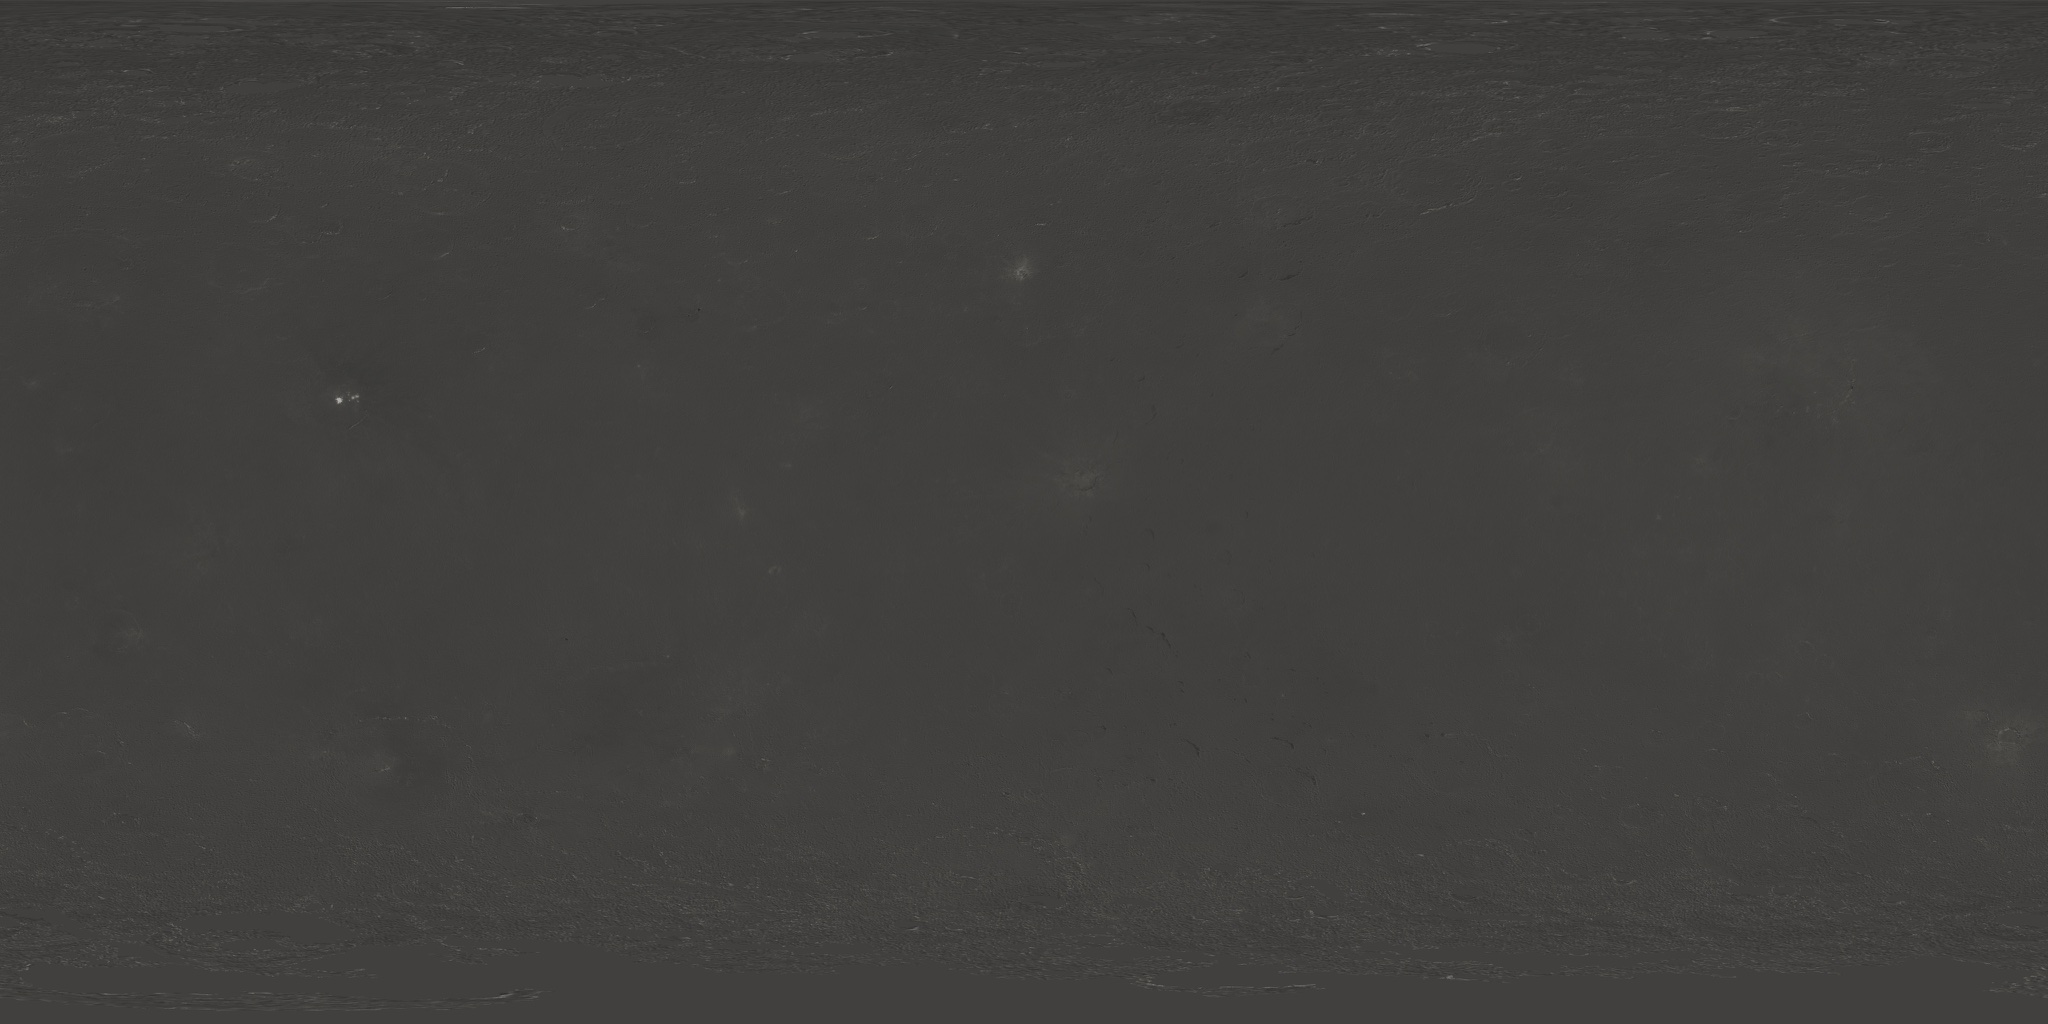
\includegraphics[width=\linewidth,height=4.4cm,keepaspectratio]{../public/textures/hd/ceres_dawn.jpg}\\[2pt]
{\scriptsize\itshape\color{orbitarMuted} Planiglob desfășurat: Harta globală a planetei pitice Ceres și a craterului Occator cu depozite strălucitoare de săruri (sonda NASA Dawn).}
\end{tabular}
\end{center}


\begin{tcolorbox}[orbitardata, title={\textbf{Repere esențiale: Ceres}}]
\small
\begin{itemize}[leftmargin=1.4em, itemsep=2pt, topsep=2pt]
  \item \textbf{Clasificare și orbită:} Planetă Pitică \quad$\bullet$\quad \textbf{Distanță:} 2,767 UA ($\approx$ 414 milioane de kilometri)
  \item \textbf{Dimensiuni și masă:} rază medie 473 de kilometri \quad$\bullet$\quad masă: 1,50e-4 $\times M_\oplus$
  \item \textbf{Gravitație și regim termic:} 0,029 $\times g_\oplus$ (0,28 m/s$^2$) \quad$\bullet$\quad temperatură medie: -105 $^\circ$C (înclinarea axei: Nespecificată)
  \item \textbf{Ciclu orbital și rotație:} perioadă orbitală (an): 1.682 zile ($\approx$ 4,61 ani pământești) \quad$\bullet$\quad rotație (zi): 9,07 ore (0,38 zile pământești) (elemente kepleriene: $a = 2,767$ UA, $e = 0,0760$, $i = 10,59^\circ$, $\Omega = 80,3^\circ$, $\omega = 73,6^\circ$)
  \item \textbf{Durata călătoriei de pe Pământ:} cu viteza luminii ($1c$): \emph{22 de minute}; cu racheta ($50.000$ de kilometri pe oră): \emph{1,5--3 ani}; cu avionul ($900$ de kilometri pe oră): \emph{33 de ani}; cu mașina ($100$ de kilometri pe oră): \emph{300 de ani}.
  \item \textbf{Repere de scară și curiozitate:} Dacă toți asteroizii din centură ar fi adunați într-o găleată, Ceres singură ar umple o treime din găleată! În craterul Occator de pe Ceres strălucesc pete albe misterioase, făcute din sare lăsată în urmă de izvoare sărate!
\end{itemize}
\end{tcolorbox}

\subsubsection*{Prezentare generală și profil astrofizic}
Descoperită la 1 ianuarie 1801 de Giuseppe Piazzi, Ceres este singura planetă pitică situată în Sistemul Solar interior. Reprezintă o protoplanetă embrionară bogată în apă și argile amoniacale. Ceres este cea mai mare lume din Centura de Asteroizi dintre Marte și Jupiter! Este atât de mare încât propria ei gravitație a modelat-o într-o sferă. Dacă toți asteroizii din centură ar fi adunați într-o găleată, Ceres singură ar umple o treime din găleată!

\subsubsection*{Alcătuirea fizică și structura internă}
Privind în profunzimea sa, alcătuirea fizică este organizată pe mai multe straturi și regiuni distincte, fiecare având un rol bine definit în evoluția și dinamica acestui obiect cosmic. În primul rând se remarcă \textbf{Nucleu stâncos hidratat}, compus din silicați și minerale argiloase. În strânsă legătură cu această componentă se află \textbf{Manta bogată în gheață și saramură}, rezervoare subterane de apă sărată care alimentează criovulcanismul (ex. muntele Ahuna Mons). În completarea acestui ansamblu întâlnim \textbf{Crustă întunecată cu depozite de carbonat de sodiu}, unde petele luminoase (faculae) din craterul Occator sunt depozite de săruri hidrotermale.

\subsubsection*{Observații astronomice și istoricul explorării}
A fost prima planetă pitică vizitată și orbitată de o sondă spațială: misiunea NASA Dawn (2015--2018). În craterul Occator de pe Ceres strălucesc pete albe misterioase, făcute din sare lăsată în urmă de izvoare sărate!

\vspace{6pt}
\begin{tcolorbox}[orbitarquiz, title={\textbf{Întrebare de verificare \#32: Ceres}}]
\textbf{Unde se află planeta pitică Ceres?}
\begin{itemize}[leftmargin=2.2em, itemsep=2pt, topsep=4pt]
  \item[$\square$ \textbf{A.}] Dincolo de Neptun, în Centura Kuiper
  \item[$\square$ \textbf{B.}] În Centura Principală de Asteroizi, între Marte și Jupiter
  \item[$\square$ \textbf{C.}] Pe orbita Pământului
  \item[$\square$ \textbf{D.}] Între Mercur și Venus
\end{itemize}
\vspace{2pt}
{\footnotesize\color{orbitarMuted}\textbf{Răspuns corect:} \textbf{B} (În Centura Principală de Asteroizi, între Marte și Jupiter). \emph{Ceres orbitează la 2,77 UA de Soare, în mijlocul Centurii Principale de Asteroizi dintre Marte și Jupiter.}}
\end{tcolorbox}
\clearpage


\subsection{Pluto}
\label{sec:body-pluto}
\vspace{-4pt}
{\large\itshape\color{orbitarAccent} Regele planetelor pitice din Centura Kuiper}\\[4pt]


\begin{center}
\begin{tabular}{@{}m{0.44\textwidth}@{\hspace{0.03\textwidth}}m{0.51\textwidth}@{}}
\centering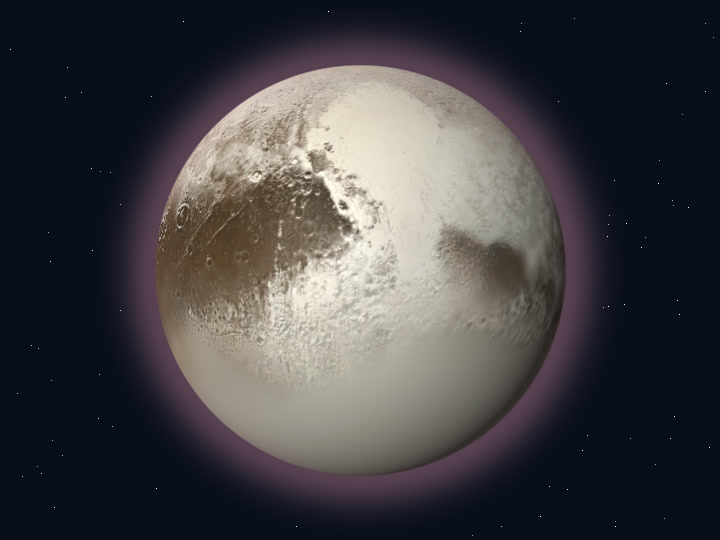
\includegraphics[width=\linewidth,height=4.4cm,keepaspectratio]{imagini/globuri/pluto.jpg}\\[2pt]
{\scriptsize\itshape\color{orbitarMuted} Vedere 3D a corpului ceresc (\textbf{Pluto})}
&
\centering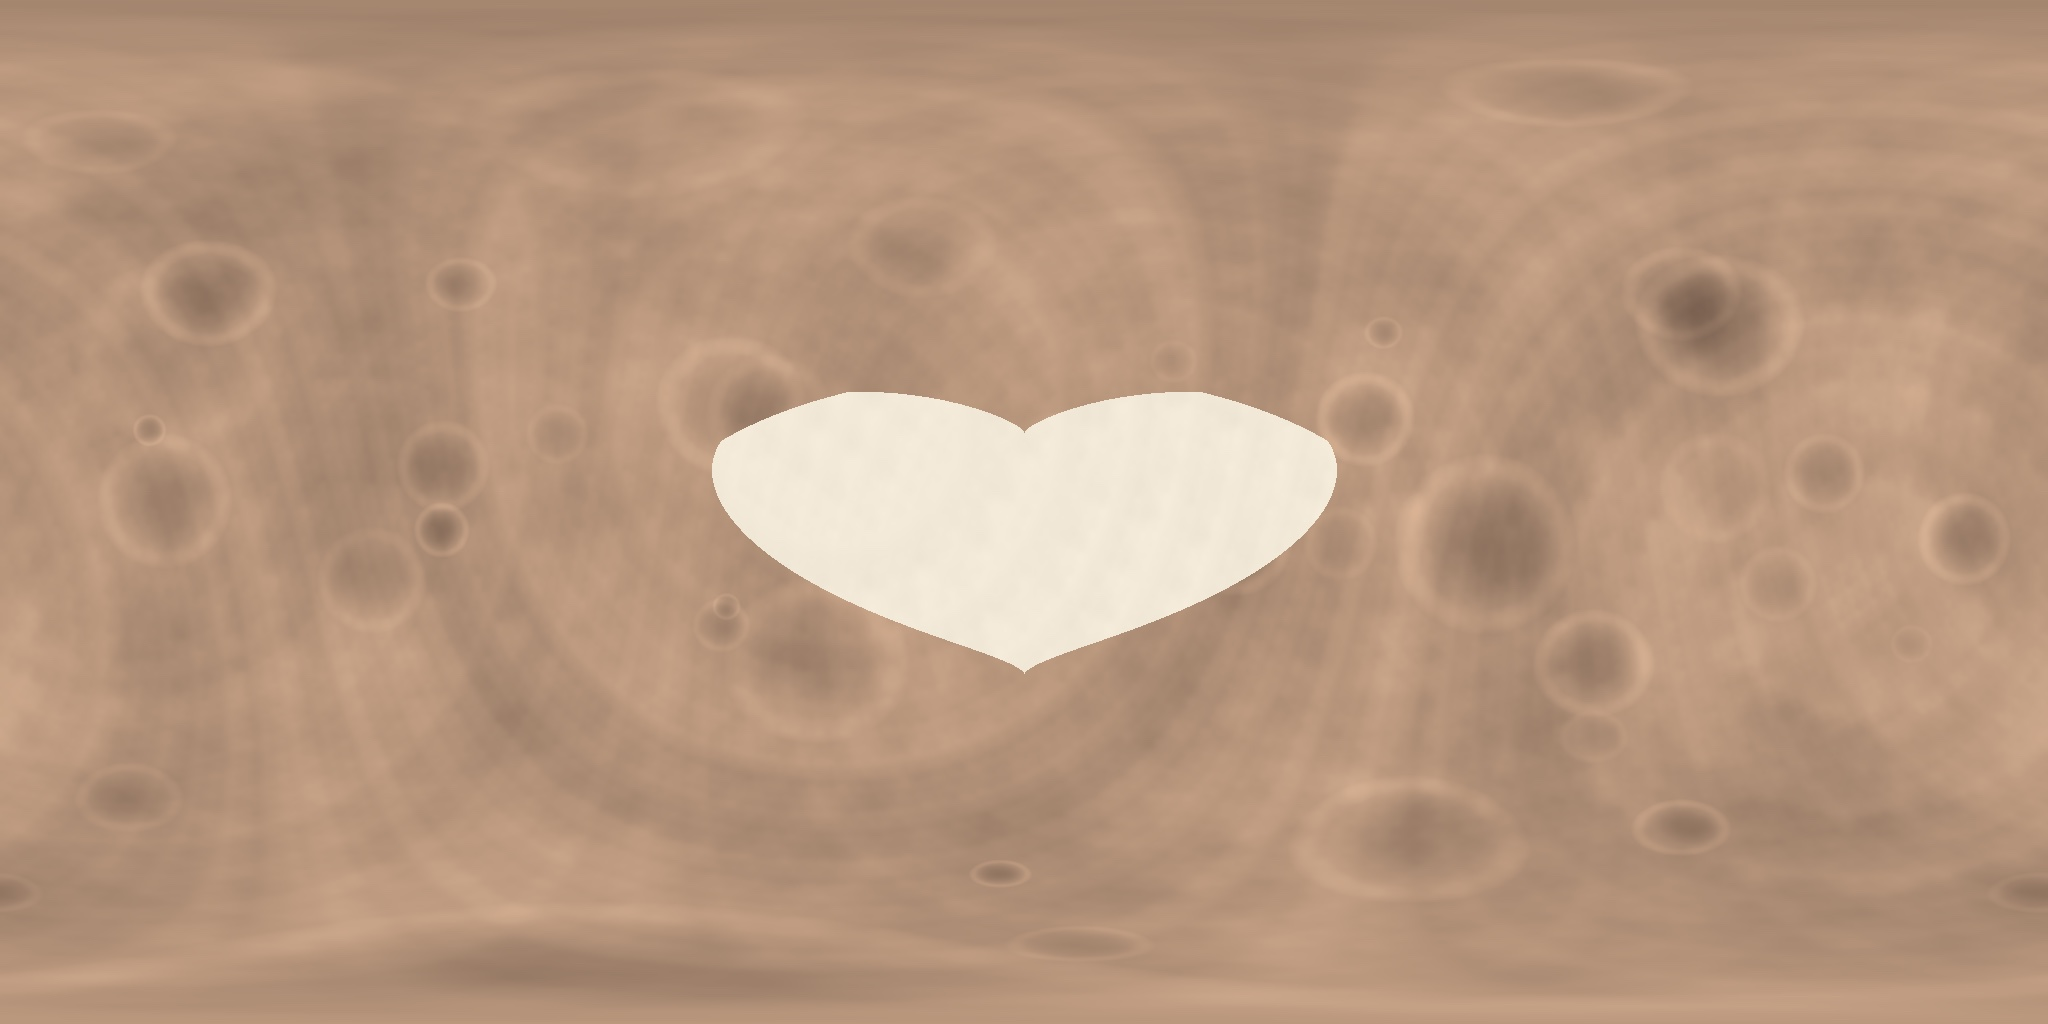
\includegraphics[width=\linewidth,height=4.4cm,keepaspectratio]{../public/textures/hd/pluto_newhorizons.jpg}\\[2pt]
{\scriptsize\itshape\color{orbitarMuted} Planiglob desfășurat: Harta globală a planetei pitice Pluto și a ghețarului în formă de inimă Tombaugh Regio / Sputnik Planitia (NASA New Horizons).}
\end{tabular}
\end{center}


\begin{tcolorbox}[orbitardata, title={\textbf{Repere esențiale: Pluto}}]
\small
\begin{itemize}[leftmargin=1.4em, itemsep=2pt, topsep=2pt]
  \item \textbf{Clasificare și orbită:} Planetă Pitică \quad$\bullet$\quad \textbf{Distanță:} 39,480 UA ($\approx$ 5.906 milioane de kilometri)
  \item \textbf{Dimensiuni și masă:} rază medie 1.188,3 de kilometri \quad$\bullet$\quad masă: 0,002 $\times M_\oplus$
  \item \textbf{Gravitație și regim termic:} 0,063 $\times g_\oplus$ (0,62 m/s$^2$) \quad$\bullet$\quad temperatură medie: -229 $^\circ$C (înclinarea axei: 122,53$^\circ$)
  \item \textbf{Ciclu orbital și rotație:} perioadă orbitală (an): 90.560 zile ($\approx$ 247,94 ani pământești) \quad$\bullet$\quad rotație (zi): 153,30 ore (Rotație retrogradă!)
  \item \textbf{Durata călătoriei de pe Pământ:} cu viteza luminii ($1c$): \emph{5 ore și 30 de minute}; cu racheta ($50.000$ de kilometri pe oră): \emph{9 ani și jumătate (New Horizons)}; cu avionul ($900$ de kilometri pe oră): \emph{720 de ani}; cu mașina ($100$ de kilometri pe oră): \emph{6.500 de ani}.
  \item \textbf{Repere de scară și curiozitate:} Pluto este mai mic chiar și decât Luna noastră, măsurând cam cât jumătate din lățimea Europei! Pluto și satelitul său cel mai mare, Charon, sunt atât de apropiați ca mărime încât dansează unul în jurul celuilalt!
\end{itemize}
\end{tcolorbox}

\subsubsection*{Prezentare generală și profil astrofizic}
Descoperită de Clyde Tombaugh în 1930 și reclasificată în 2006 de UAI drept planetă pitică (obiect plutoid din Centura Kuiper), Pluto are o orbită excentrică și înclinată la 17$^\circ$ și o geologie surprinzător de activă, cu munți de gheață de apă și ghețari de azot. Pluto este o planetă pitică îndepărtată și înghețată care poartă pe pieptul ei o formă uriașă de inimă albă din gheață de azot! Pluto este mai mic chiar și decât Luna noastră, măsurând cam cât jumătate din lățimea Europei!

\subsubsection*{Alcătuirea fizică și structura internă}
Privind în profunzimea sa, alcătuirea fizică este organizată pe mai multe straturi și regiuni distincte, fiecare având un rol bine definit în evoluția și dinamica acestui obiect cosmic. În primul rând se remarcă \textbf{Nucleu stâncos (70\% din diametru)}, bogat în silicați, a cărui dezintegrare radioactivă menține căldura internă. În strânsă legătură cu această componentă se află \textbf{Manta de gheață de apă ( și posibil ocean subteran)}, care susține lanțuri muntoase înalte de 3--4 kilometri. În completarea acestui ansamblu întâlnim \textbf{Suprafață de azot, metan și CO înghețat}, dominată de câmpia convectivă Sputnik Planitia (\guillemotleft{}Inima lui Pluto\guillemotright{}).

\subsubsection*{Observații astronomice și istoricul explorării}
Survolată în premieră istorică la 14 iulie 2015 de sonda NASA New Horizons, care a dezvăluit munți și câmpii de gheață tinere. Pluto și satelitul său cel mai mare, Charon, sunt atât de apropiați ca mărime încât dansează unul în jurul celuilalt!

\vspace{6pt}
\begin{tcolorbox}[orbitarquiz, title={\textbf{Întrebare de verificare \#33: Pluto}}]
\textbf{Cum se numește celebra regiune strălucitoare în formă de inimă de pe Pluto?}
\begin{itemize}[leftmargin=2.2em, itemsep=2pt, topsep=4pt]
  \item[$\square$ \textbf{A.}] Tombaugh Regio (Sputnik Planitia)
  \item[$\square$ \textbf{B.}] Olympus Mons
  \item[$\square$ \textbf{C.}] Mare Tranquillitatis
  \item[$\square$ \textbf{D.}] Caloris Planitia
\end{itemize}
\vspace{2pt}
{\footnotesize\color{orbitarMuted}\textbf{Răspuns corect:} \textbf{A} (Tombaugh Regio (Sputnik Planitia)). \emph{Regiunea în formă de inimă a fost numită Tombaugh Regio în onoarea descoperitorului lui Pluto, iar lobul ei vestic este ghețarul Sputnik Planitia.}}
\end{tcolorbox}
\clearpage


\subsection{Charon}
\label{sec:body-charon}
\vspace{-4pt}
{\large\itshape\color{orbitarAccent} Satelitul-pereche al lui Pluto, cu calota roșiatică Mordor Macula}\\[4pt]


\begin{center}
\begin{tabular}{@{}m{0.44\textwidth}@{\hspace{0.03\textwidth}}m{0.51\textwidth}@{}}
\centering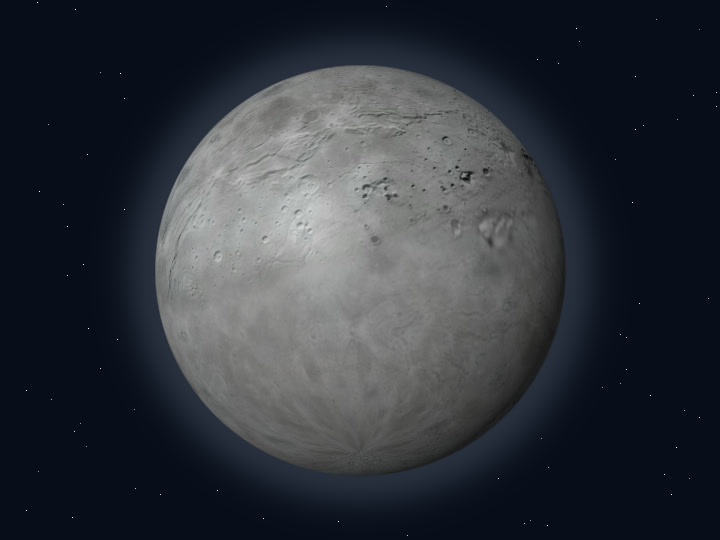
\includegraphics[width=\linewidth,height=4.4cm,keepaspectratio]{imagini/globuri/charon.jpg}\\[2pt]
{\scriptsize\itshape\color{orbitarMuted} Vedere 3D a corpului ceresc (\textbf{Charon})}
&
\centering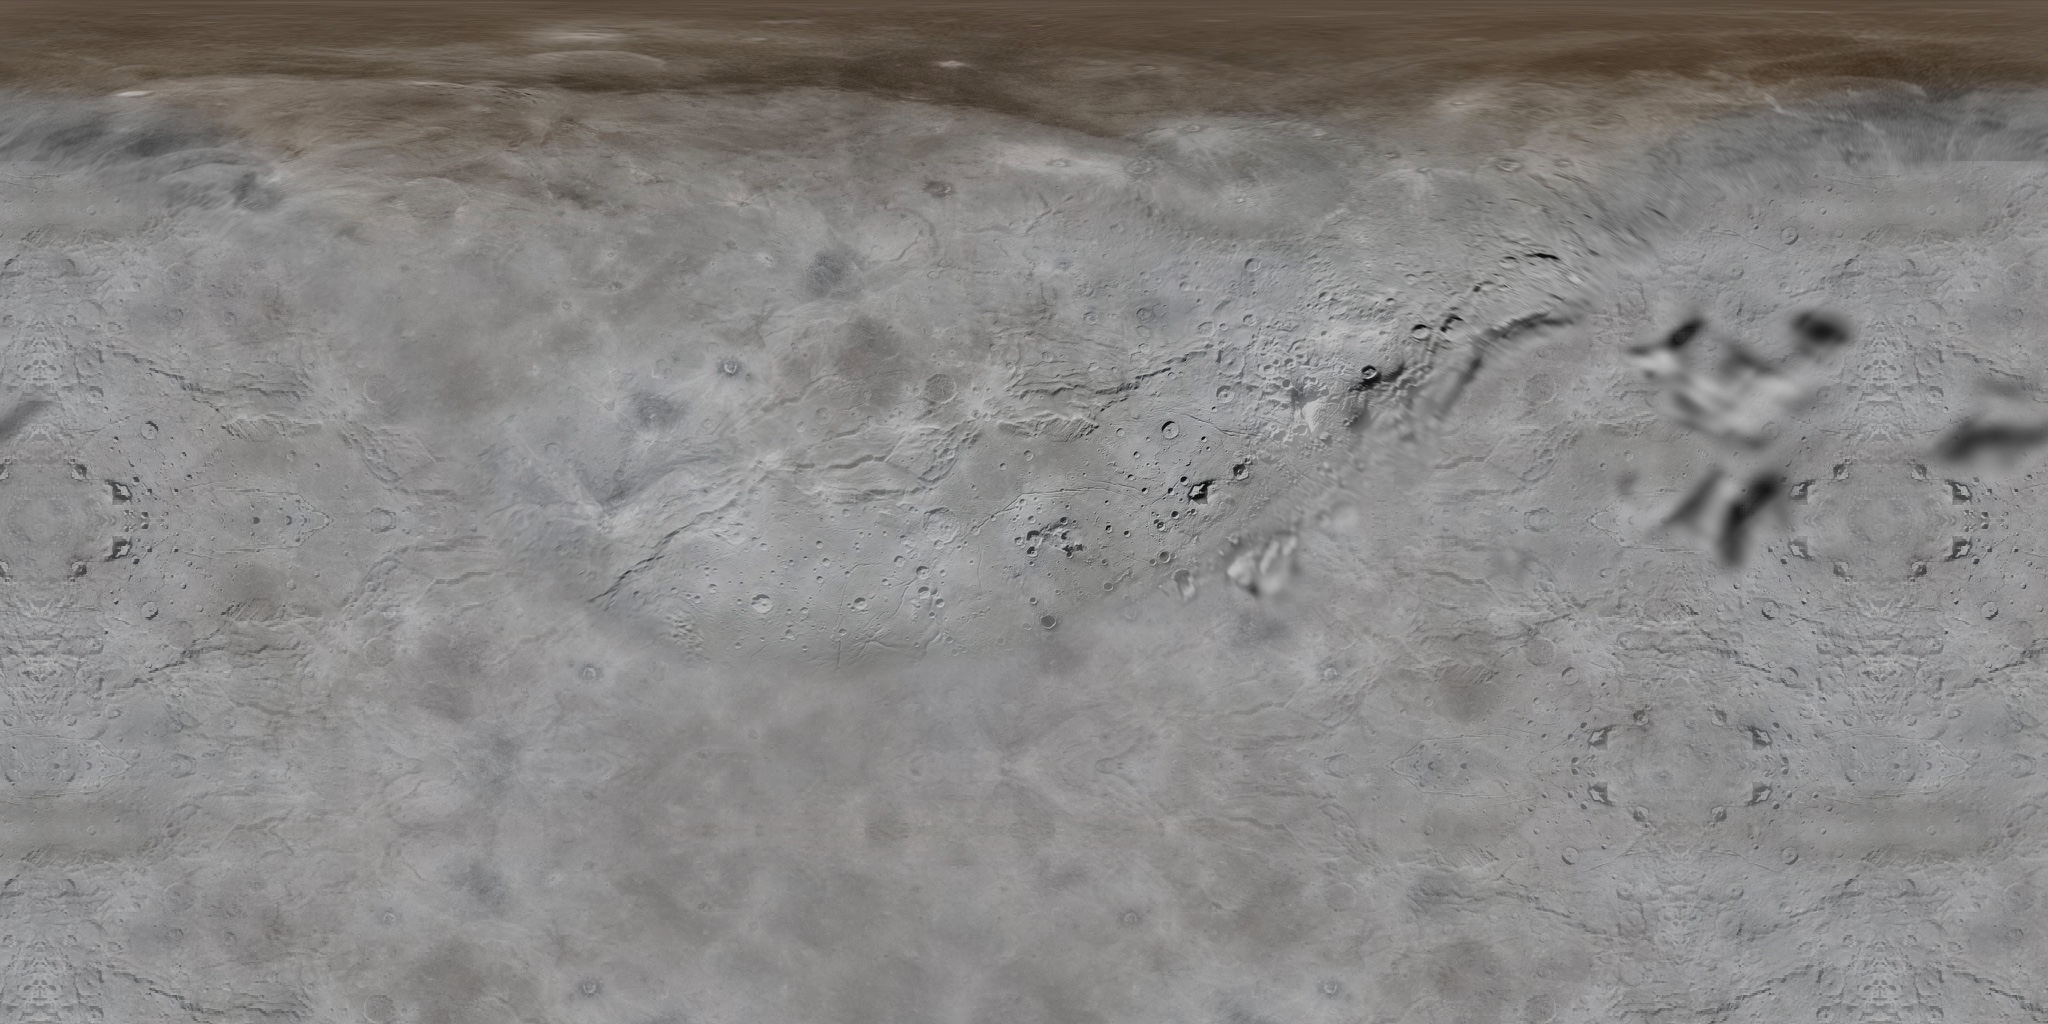
\includegraphics[width=\linewidth,height=4.4cm,keepaspectratio]{../public/textures/hd/charon_newhorizons.jpg}\\[2pt]
{\scriptsize\itshape\color{orbitarMuted} Planiglob desfășurat: Harta lunii Charon cu calota polară roșiatică Mordor Macula și canionul Serenity Chasma (NASA New Horizons, 2015).}
\end{tabular}
\end{center}


\begin{tcolorbox}[orbitardata, title={\textbf{Repere esențiale: Charon}}]
\small
\begin{itemize}[leftmargin=1.4em, itemsep=2pt, topsep=2pt]
  \item \textbf{Clasificare și orbită:} Satelit Natural (Lună) (orbitează în jurul: \textbf{Pluto}) \quad$\bullet$\quad \textbf{Distanță:} 39,480 UA ($\approx$ 5.906 milioane de kilometri)
  \item \textbf{Dimensiuni și masă:} rază medie 606 kilometri \quad$\bullet$\quad masă: 2,66e-4 $\times M_\oplus$
  \item \textbf{Gravitație și regim termic:} 0,029 $\times g_\oplus$ (0,28 m/s$^2$) \quad$\bullet$\quad temperatură medie: -220 $^\circ$C (înclinarea axei: Nespecificată)
  \item \textbf{Ciclu orbital și rotație:} perioadă orbitală (an): 6,387 zile pământești \quad$\bullet$\quad rotație (zi): 153,30 ore (6,39 zile pământești)
  \item \textbf{Durata călătoriei de pe Pământ:} cu viteza luminii ($1c$): \emph{5 ore și 30 de minute}; cu racheta ($50.000$ de kilometri pe oră): \emph{9 ani și jumătate (New Horizons)}; cu avionul ($900$ de kilometri pe oră): \emph{720 de ani}; cu mașina ($100$ de kilometri pe oră): \emph{6.500 de ani}.
  \item \textbf{Repere de scară și curiozitate:} Charon poartă la polul său nordic o \guillemotleft{}căciulă\guillemotright{} roșiatică de gheață colorată, iar pe la mijloc are un brâu de canioane uriașe! Dacă ai locui pe partea lui Pluto îndreptată spre Charon, ai vedea luna Charon stând nemișcată în exact același loc pe cer zi și noapte!
\end{itemize}
\end{tcolorbox}

\subsubsection*{Prezentare generală și profil astrofizic}
Descoperită în 1978 de James Christy, Charon are o rază de 606 kilometri (peste jumătate din diametrul lui Pluto). Centrul de masă comun (baricentrul) se află în spațiul liber dintre cele două corpuri, motiv pentru care sistemul Pluto--Charon este adesea numit o planetă pitică dublă. Charon este cel mai bun prieten al lui Pluto! Este atât de mare în comparație cu Pluto încât cei doi stau mereu față în față pe cer, ca doi dansatori care se țin de mâini. Charon poartă la polul său nordic o \guillemotleft{}căciulă\guillemotright{} roșiatică de gheață colorată, iar pe la mijloc are un brâu de canioane uriașe!

\subsubsection*{Alcătuirea fizică și structura internă}
Privind în profunzimea sa, alcătuirea fizică este organizată pe mai multe straturi și regiuni distincte, fiecare având un rol bine definit în evoluția și dinamica acestui obiect cosmic. În primul rând se remarcă \textbf{Interior de rocă (55\%) și gheață de apă (45\%)}, unde spre deosebire de Pluto, suprafața lui Charon este dominată de gheață de apă cristalină și hidrați de amoniac. În strânsă legătură cu această componentă se află \textbf{Serenity Chasma și centura de canioane}, un lanț de canioane lung de peste 1.000 de kilometri și adânc de 7--9 kilometri, format când un ocean subteran străvechi a înghețat și s-a extins. În completarea acestui ansamblu întâlnim \textbf{Calota polară Mordor Macula}, regiune polară roșiatică formată din metan scăpat din atmosfera lui Pluto, captat de polul rece al lui Charon și transformat în toline de razele UV.

\subsubsection*{Observații astronomice și istoricul explorării}
Fotografiată la rezoluție înaltă de sonda NASA New Horizons la 14 iulie 2015. Dacă ai locui pe partea lui Pluto îndreptată spre Charon, ai vedea luna Charon stând nemișcată în exact același loc pe cer zi și noapte!

\vspace{6pt}
\begin{tcolorbox}[orbitarquiz, title={\textbf{Întrebare de verificare \#34: Charon}}]
\textbf{De ce stau Pluto și Charon mereu cu aceeași față îndreptată unul spre celălalt?}
\begin{itemize}[leftmargin=2.2em, itemsep=2pt, topsep=4pt]
  \item[$\square$ \textbf{A.}] Ambele corpuri sunt în rotație sincronă reciprocă (blocare mareică dublă)
  \item[$\square$ \textbf{B.}] Pentru că sunt lipite între ele
  \item[$\square$ \textbf{C.}] Pentru că nu se rotesc deloc
  \item[$\square$ \textbf{D.}] Din cauza câmpului magnetic al lui Neptun
\end{itemize}
\vspace{2pt}
{\footnotesize\color{orbitarMuted}\textbf{Răspuns corect:} \textbf{A} (Ambele corpuri sunt în rotație sincronă reciprocă (blocare mareică dublă)). \emph{Pluto și Charon se rotesc în jurul axelor lor în exact 6,387 zile, având exact aceeași durată în care orbitează în jurul baricentrului lor comun.}}
\end{tcolorbox}
\clearpage


\subsection{Haumea}
\label{sec:body-haumea}
\vspace{-4pt}
{\large\itshape\color{orbitarAccent} Planeta pitică ovală cu inel propriu și rotație ultra-rapidă}\\[4pt]


\begin{center}
\begin{tabular}{@{}m{0.44\textwidth}@{\hspace{0.03\textwidth}}m{0.51\textwidth}@{}}
\centering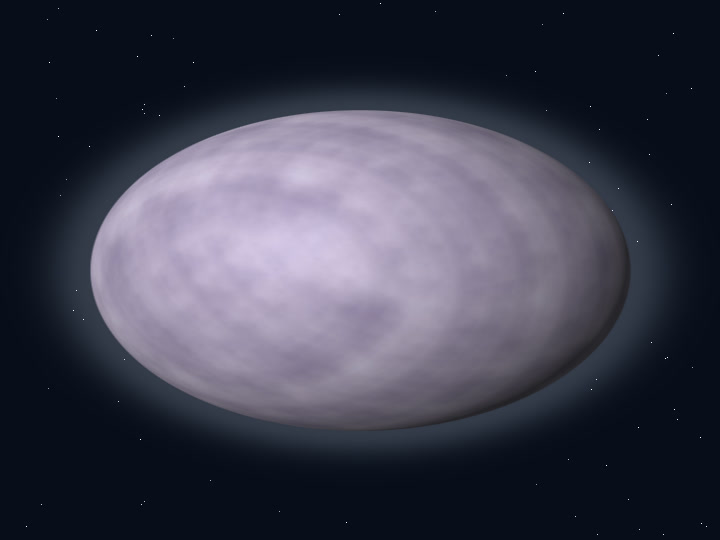
\includegraphics[width=\linewidth,height=4.4cm,keepaspectratio]{imagini/globuri/haumea.jpg}\\[2pt]
{\scriptsize\itshape\color{orbitarMuted} Vedere 3D a corpului ceresc (\textbf{Haumea})}
&
\centering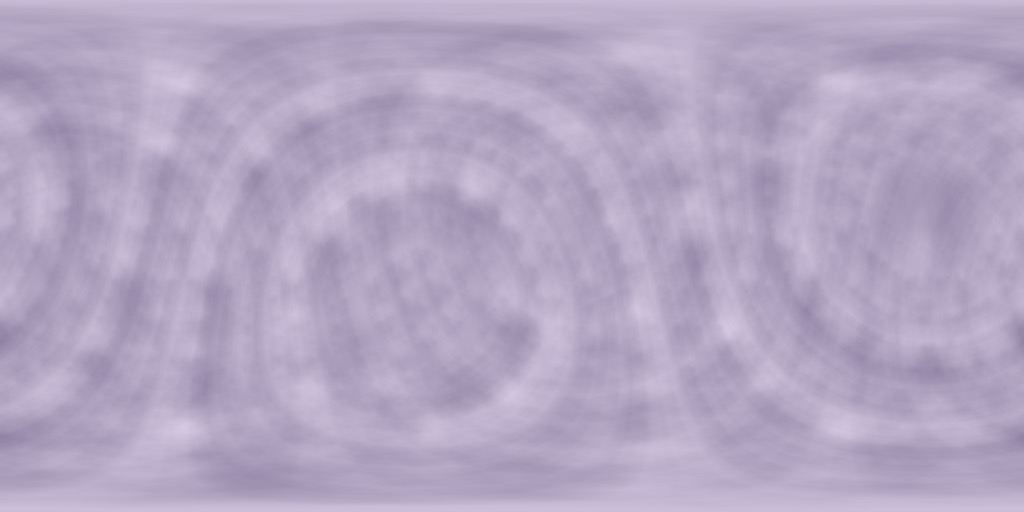
\includegraphics[width=\linewidth,height=4.4cm,keepaspectratio]{../public/textures/haumea.jpg}\\[2pt]
{\scriptsize\itshape\color{orbitarMuted} Planiglob desfășurat: Harta suprafeței de gheață cristalină și a petei roșiatice de pe planeta pitică elipsoidală Haumea.}
\end{tabular}
\end{center}


\begin{tcolorbox}[orbitardata, title={\textbf{Repere esențiale: Haumea}}]
\small
\begin{itemize}[leftmargin=1.4em, itemsep=2pt, topsep=2pt]
  \item \textbf{Clasificare și orbită:} Planetă Pitică \quad$\bullet$\quad \textbf{Distanță:} 43,130 UA ($\approx$ 6.452 milioane de kilometri)
  \item \textbf{Dimensiuni și masă:} rază medie 780 de kilometri \quad$\bullet$\quad masă: 6,70e-4 $\times M_\oplus$
  \item \textbf{Gravitație și regim termic:} 0,041 $\times g_\oplus$ (0,40 m/s$^2$) \quad$\bullet$\quad temperatură medie: -241 $^\circ$C (înclinarea axei: Nespecificată)
  \item \textbf{Ciclu orbital și rotație:} perioadă orbitală (an): 103.774 zile ($\approx$ 284,12 ani pământești) \quad$\bullet$\quad rotație (zi): 3,92 ore (0,16 zile pământești) (elemente kepleriene: $a = 43,130$ UA, $e = 0,1950$, $i = 28,19^\circ$, $\Omega = 122,1^\circ$, $\omega = 239,0^\circ$)
  \item \textbf{Durata călătoriei de pe Pământ:} cu viteza luminii ($1c$): \emph{6 ore}; cu racheta ($50.000$ de kilometri pe oră): \emph{14 ani}; cu avionul ($900$ de kilometri pe oră): \emph{790 de ani}; cu mașina ($100$ de kilometri pe oră): \emph{7.100 de ani}.
  \item \textbf{Repere de scară și curiozitate:} Haumea are forma unei pietre plate de râu sau a unui ou alb de Paște care se învârte amețitor! Haumea are două luni mici (Hi'iaka și Namaka) și chiar și un inel subțire în jurul ei, ca un mini-Saturn!
\end{itemize}
\end{tcolorbox}

\subsubsection*{Prezentare generală și profil astrofizic}
Situată în Centura Kuiper la aproximativ 43 UA, Haumea are forma unui elipsoid triaxial (aproximativ 2.100 $\times$ 1.680 $\times$ 1.070 de kilometri) din cauza perioadei de rotație de doar 3,9 ore. În 2017, printr-o ocultație stelară, s-a descoperit că posedă un sistem de inele. Haumea este cel mai rapid titirez mare din Sistemul Solar! O zi pe Haumea durează mai puțin de 4 ore, iar din această cauză s-a alungit ca o minge de rugby! Haumea are forma unei pietre plate de râu sau a unui ou alb de Paște care se învârte amețitor!

\subsubsection*{Alcătuirea fizică și structura internă}
Privind în profunzimea sa, alcătuirea fizică este organizată pe mai multe straturi și regiuni distincte, fiecare având un rol bine definit în evoluția și dinamica acestui obiect cosmic. În primul rând se remarcă \textbf{Interior stâncos diferențiat}, densitate ridicată (aproximativ 2,0 g/cm$^3$) rezultată după un impact antic care i-a accelerat rotația. În strânsă legătură cu această componentă se află \textbf{Crustă subțire de gheață cristalină pură}, unde spre deosebire de alte obiecte transneptuniene, suprafața ei este acoperită cu gheață de apă cristalină. În completarea acestui ansamblu întâlnim \textbf{Inel ecuatorial (rază aproximativ 2.287 de kilometri)}, primul inel descoperit în jurul unui obiect transneptunian.

\subsubsection*{Observații astronomice și istoricul explorării}
Descoperită în 2004 și caracterizată prin ocultații stelare și observații ale telescoapelor spațiale. Haumea are două luni mici (Hi'iaka și Namaka) și chiar și un inel subțire în jurul ei, ca un mini-Saturn!

\vspace{6pt}
\begin{tcolorbox}[orbitarquiz, title={\textbf{Întrebare de verificare \#35: Haumea}}]
\textbf{De ce are planeta pitică Haumea o formă alungită, asemănătoare unei mingi de rugby?}
\begin{itemize}[leftmargin=2.2em, itemsep=2pt, topsep=4pt]
  \item[$\square$ \textbf{A.}] Din cauza căldurii Soarelui
  \item[$\square$ \textbf{B.}] Din cauza rotației extrem de rapide (o rotație completă în mai puțin de 4 ore)
  \item[$\square$ \textbf{C.}] Pentru că este atrasă de Marte
  \item[$\square$ \textbf{D.}] Pentru că este făcută din gaz
\end{itemize}
\vspace{2pt}
{\footnotesize\color{orbitarMuted}\textbf{Răspuns corect:} \textbf{B} (Din cauza rotației extrem de rapide (o rotație completă în mai puțin de 4 ore)). \emph{Forța centrifugă produsă de rotația în doar 3,9 ore i-a deformat corpul într-un elipsoid alungit.}}
\end{tcolorbox}
\clearpage


\subsection{Makemake}
\label{sec:body-makemake}
\vspace{-4pt}
{\large\itshape\color{orbitarAccent} Lumea roșiatică de metan înghețat din Centura Kuiper}\\[4pt]


\begin{center}
\begin{tabular}{@{}m{0.44\textwidth}@{\hspace{0.03\textwidth}}m{0.51\textwidth}@{}}
\centering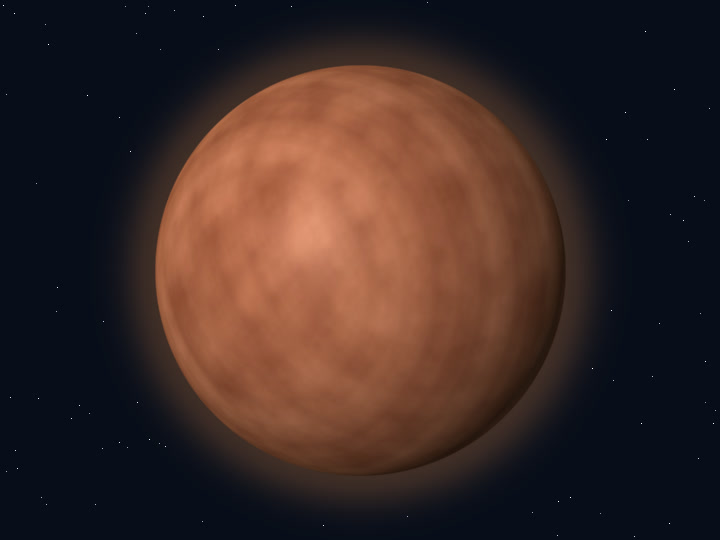
\includegraphics[width=\linewidth,height=4.4cm,keepaspectratio]{imagini/globuri/makemake.jpg}\\[2pt]
{\scriptsize\itshape\color{orbitarMuted} Vedere 3D a corpului ceresc (\textbf{Makemake})}
&
\centering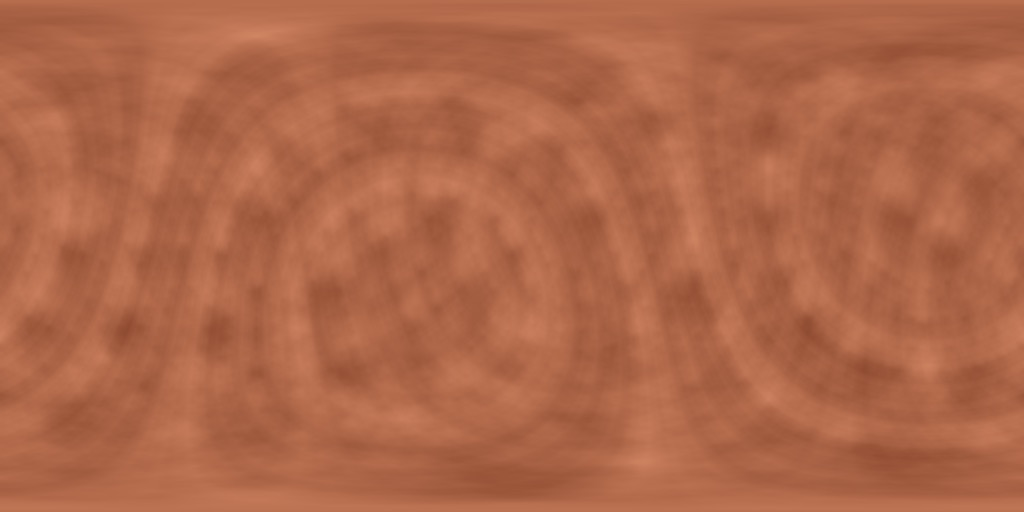
\includegraphics[width=\linewidth,height=4.4cm,keepaspectratio]{../public/textures/makemake.jpg}\\[2pt]
{\scriptsize\itshape\color{orbitarMuted} Planiglob desfășurat: Harta suprafeței bogate în toline roșiatice și metan înghețat a planetei pitice Makemake din Centura Kuiper.}
\end{tabular}
\end{center}


\begin{tcolorbox}[orbitardata, title={\textbf{Repere esențiale: Makemake}}]
\small
\begin{itemize}[leftmargin=1.4em, itemsep=2pt, topsep=2pt]
  \item \textbf{Clasificare și orbită:} Planetă Pitică \quad$\bullet$\quad \textbf{Distanță:} 45,430 UA ($\approx$ 6.796 milioane de kilometri)
  \item \textbf{Dimensiuni și masă:} rază medie 715 kilometri \quad$\bullet$\quad masă: 5,00e-4 $\times M_\oplus$
  \item \textbf{Gravitație și regim termic:} 0,050 $\times g_\oplus$ (0,49 m/s$^2$) \quad$\bullet$\quad temperatură medie: -243 $^\circ$C (înclinarea axei: Nespecificată)
  \item \textbf{Ciclu orbital și rotație:} perioadă orbitală (an): 111.845 zile ($\approx$ 306,21 ani pământești) \quad$\bullet$\quad rotație (zi): 22,83 ore (0,95 zile pământești) (elemente kepleriene: $a = 45,430$ UA, $e = 0,1610$, $i = 28,98^\circ$, $\Omega = 79,6^\circ$, $\omega = 294,8^\circ$)
  \item \textbf{Durata călătoriei de pe Pământ:} cu viteza luminii ($1c$): \emph{6 ore și 18 minute}; cu racheta ($50.000$ de kilometri pe oră): \emph{15 ani}; cu avionul ($900$ de kilometri pe oră): \emph{830 de ani}; cu mașina ($100$ de kilometri pe oră): \emph{7.500 de ani}.
  \item \textbf{Repere de scară și curiozitate:} Makemake este ca un bulgăre mare de înghețată de căpșuni la marginea Sistemului Solar! A fost descoperită chiar în zilele de după Paște în anul 2005, așa că porecla ei inițială a fost \guillemotleft{}Iepurașul de Paște\guillemotright{} (Easterbunny)!
\end{itemize}
\end{tcolorbox}

\subsubsection*{Prezentare generală și profil astrofizic}
A doua planetă pitică ca strălucire din Centura Kuiper (după Pluto), Makemake orbitează la o distanță medie de 45,4 UA în 306 ani terestri. Are o suprafață bogată în pelete de metan și etan înghețat și un mic satelit întunecat botezat MK 2. Makemake este unul dintre cele mai strălucitoare obiecte din Centura Kuiper, numit după zeul primăverii și al fertilității din Insula Paștelui! Makemake este ca un bulgăre mare de înghețată de căpșuni la marginea Sistemului Solar!

\subsubsection*{Alcătuirea fizică și structura internă}
Privind în profunzimea sa, alcătuirea fizică este organizată pe mai multe straturi și regiuni distincte, fiecare având un rol bine definit în evoluția și dinamica acestui obiect cosmic. În primul rând se remarcă \textbf{Nucleu de silicați și gheață}, interior rece compus dintr-un amestec de rocă și gheață de apă. În strânsă legătură cu această componentă se află \textbf{Suprafață acoperită cu metan, etan și toline}, unde radiația UV solară transformă metanul în compuși organici roșiatici (toline). În completarea acestui ansamblu întâlnim \textbf{Exosferă sezonieră infimă}, unde ocultațiile stelare arată că Makemake nu posedă o atmosferă globală substanțială.

\subsubsection*{Observații astronomice și istoricul explorării}
Descoperită în martie 2005 la Observatorul Palomar; satelitul său MK 2 a fost descoperit cu Telescopul Hubble în 2016. A fost descoperită chiar în zilele de după Paște în anul 2005, așa că porecla ei inițială a fost \guillemotleft{}Iepurașul de Paște\guillemotright{} (Easterbunny)!

\vspace{6pt}
\begin{tcolorbox}[orbitarquiz, title={\textbf{Întrebare de verificare \#36: Makemake}}]
\textbf{Care a fost porecla dată de astronomi planetei pitice Makemake la descoperire?}
\begin{itemize}[leftmargin=2.2em, itemsep=2pt, topsep=4pt]
  \item[$\square$ \textbf{A.}] Moș Crăciun
  \item[$\square$ \textbf{B.}] Iepurașul de Paște (Easterbunny)
  \item[$\square$ \textbf{C.}] Micul Prinț
  \item[$\square$ \textbf{D.}] Steaua Polară
\end{itemize}
\vspace{2pt}
{\footnotesize\color{orbitarMuted}\textbf{Răspuns corect:} \textbf{B} (Iepurașul de Paște (Easterbunny)). \emph{Fiind descoperită la scurt timp după Paștele anului 2005, echipa a poreclit-o \guillemotleft{}Easterbunny\guillemotright{}, iar numele oficial Makemake provine din mitologia Rapa Nui (Insula Paștelui).}}
\end{tcolorbox}
\clearpage


\subsection{Eris}
\label{sec:body-eris}
\vspace{-4pt}
{\large\itshape\color{orbitarAccent} Cea mai masivă planetă pitică cunoscută, din Discul Împrăștiat}\\[4pt]


\begin{center}
\begin{tabular}{@{}m{0.44\textwidth}@{\hspace{0.03\textwidth}}m{0.51\textwidth}@{}}
\centering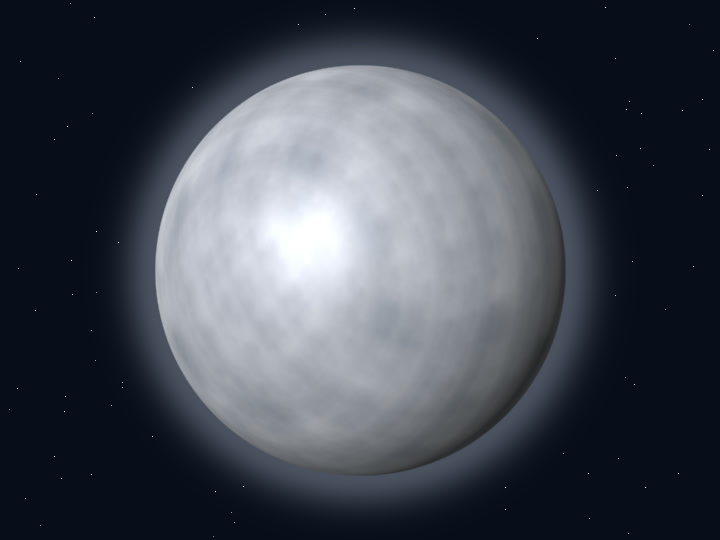
\includegraphics[width=\linewidth,height=4.4cm,keepaspectratio]{imagini/globuri/eris.jpg}\\[2pt]
{\scriptsize\itshape\color{orbitarMuted} Vedere 3D a corpului ceresc (\textbf{Eris})}
&
\centering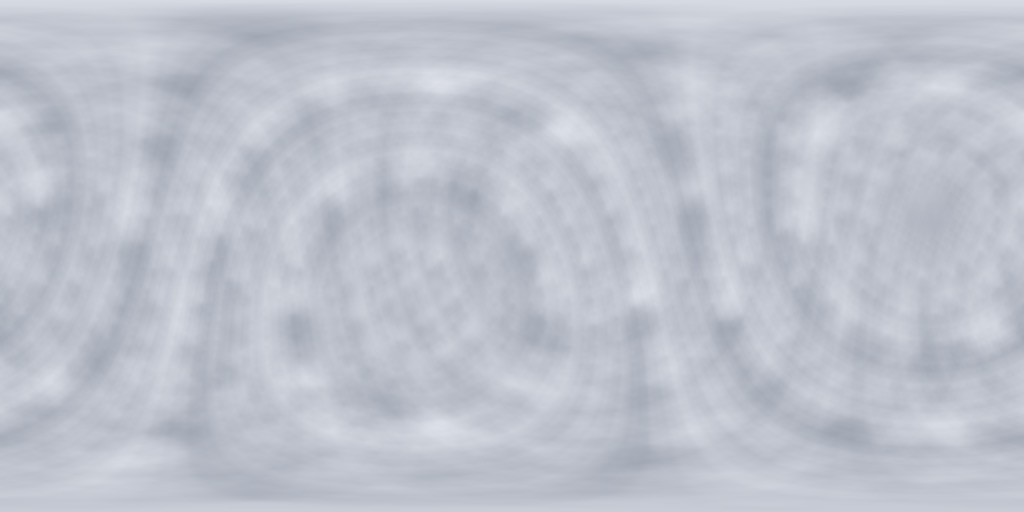
\includegraphics[width=\linewidth,height=4.4cm,keepaspectratio]{../public/textures/eris.jpg}\\[2pt]
{\scriptsize\itshape\color{orbitarMuted} Planiglob desfășurat: Harta artistică științifică a suprafeței înghețate și extrem de reflectante de metan a planetei pitice Eris.}
\end{tabular}
\end{center}


\begin{tcolorbox}[orbitardata, title={\textbf{Repere esențiale: Eris}}]
\small
\begin{itemize}[leftmargin=1.4em, itemsep=2pt, topsep=2pt]
  \item \textbf{Clasificare și orbită:} Planetă Pitică \quad$\bullet$\quad \textbf{Distanță:} 67,860 UA ($\approx$ 10.152 milioane de kilometri)
  \item \textbf{Dimensiuni și masă:} rază medie 1.163 de kilometri \quad$\bullet$\quad masă: 0,003 $\times M_\oplus$
  \item \textbf{Gravitație și regim termic:} 0,084 $\times g_\oplus$ (0,82 m/s$^2$) \quad$\bullet$\quad temperatură medie: -243 $^\circ$C (înclinarea axei: Nespecificată)
  \item \textbf{Ciclu orbital și rotație:} perioadă orbitală (an): 203.830 zile ($\approx$ 558,06 ani pământești) \quad$\bullet$\quad rotație (zi): 25,90 ore (1,08 zile pământești) (elemente kepleriene: $a = 67,860$ UA, $e = 0,4360$, $i = 44,04^\circ$, $\Omega = 35,9^\circ$, $\omega = 151,6^\circ$)
  \item \textbf{Durata călătoriei de pe Pământ:} cu viteza luminii ($1c$): \emph{9 ore și 25 de minute}; cu racheta ($50.000$ de kilometri pe oră): \emph{25 de ani}; cu avionul ($900$ de kilometri pe oră): \emph{1.200 de ani}; cu mașina ($100$ de kilometri pe oră): \emph{11.000 de ani}.
  \item \textbf{Repere de scară și curiozitate:} Eris este aproape geamănă ca mărime cu Pluto, dar cântărește puțin mai mult pentru că are mai multă piatră în interior! Pe Eris este atât de frig încât toată atmosfera ei a înghețat și s-a așternut pe sol ca o pătură sclipitoare de promoroacă!
\end{itemize}
\end{tcolorbox}

\subsubsection*{Prezentare generală și profil astrofizic}
Descoperită în 2005 de echipa lui Mike Brown la Observatorul Palomar, Eris este cu 27\% mai masivă decât Pluto. Orbita sa puternic înclinată (44$^\circ$) o poartă până la 97 UA de Soare în Discul Împrăștiat, iar un an pe Eris durează 558 de ani terestri. Eris este o lume albă ca zăpada, aflată de peste două ori mai departe de Soare decât Neptun! Descoperirea ei i-a făcut pe astronomi să inventeze categoria de \guillemotleft{}planetă pitică\guillemotright{}. Eris este aproape geamănă ca mărime cu Pluto, dar cântărește puțin mai mult pentru că are mai multă piatră în interior!

\subsubsection*{Alcătuirea fizică și structura internă}
Privind în profunzimea sa, alcătuirea fizică este organizată pe mai multe straturi și regiuni distincte, fiecare având un rol bine definit în evoluția și dinamica acestui obiect cosmic. În primul rând se remarcă \textbf{Nucleu dens de silicați}, care constituie aproximativ 85\% din masa corpului (densitate medie 2,52 g/cm$^3$). În strânsă legătură cu această componentă se află \textbf{Manta de gheață de apă}, înveliș glaciar rigid la temperaturi apropiate de zero absolut. În completarea acestui ansamblu întâlnim \textbf{Suprafață ultra-reflectivă de metan și azot înghețat}, care reflectă 96\% din lumina solară incidentă.

\subsubsection*{Observații astronomice și istoricul explorării}
Studiată prin telescoapele Hubble, Keck și James Webb, împreună cu satelitul său Dysnomia. Pe Eris este atât de frig încât toată atmosfera ei a înghețat și s-a așternut pe sol ca o pătură sclipitoare de promoroacă!

\vspace{6pt}
\begin{tcolorbox}[orbitarquiz, title={\textbf{Întrebare de verificare \#37: Eris}}]
\textbf{Ce eveniment astronomic a determinat descoperirea planetei pitice Eris în 2005?}
\begin{itemize}[leftmargin=2.2em, itemsep=2pt, topsep=4pt]
  \item[$\square$ \textbf{A.}] Lansarea telescopului Hubble
  \item[$\square$ \textbf{B.}] Definirea oficială a categoriei de \guillemotleft{}planetă pitică\guillemotright{} și reclasificarea lui Pluto în 2006
  \item[$\square$ \textbf{C.}] Asolizarea pe Marte
  \item[$\square$ \textbf{D.}] Descoperirea inelelor lui Saturn
\end{itemize}
\vspace{2pt}
{\footnotesize\color{orbitarMuted}\textbf{Răspuns corect:} \textbf{B} (Definirea oficială a categoriei de \guillemotleft{}planetă pitică\guillemotright{} și reclasificarea lui Pluto în 2006). \emph{Deoarece Eris s-a dovedit mai masivă decât Pluto, Uniunea Astronomică Internațională a stabilit în 2006 criteriile pentru planete și planete pitice.}}
\end{tcolorbox}
\clearpage


\section{Asteroizi Principali și Obiecte din Apropierea Pământului}

\subsection{4 Vesta}
\label{sec:body-vesta}
\vspace{-4pt}
{\large\itshape\color{orbitarAccent} Cel mai strălucitor asteroid și protoplanetă stâncoasă}\\[4pt]


\begin{center}
\begin{tabular}{@{}m{0.44\textwidth}@{\hspace{0.03\textwidth}}m{0.51\textwidth}@{}}
\centering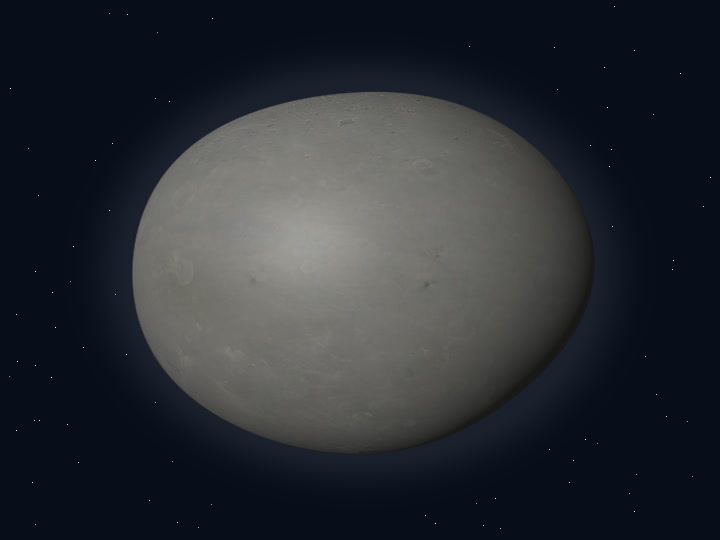
\includegraphics[width=\linewidth,height=4.4cm,keepaspectratio]{imagini/globuri/vesta.jpg}\\[2pt]
{\scriptsize\itshape\color{orbitarMuted} Vedere 3D a corpului ceresc (\textbf{4 Vesta})}
&
\centering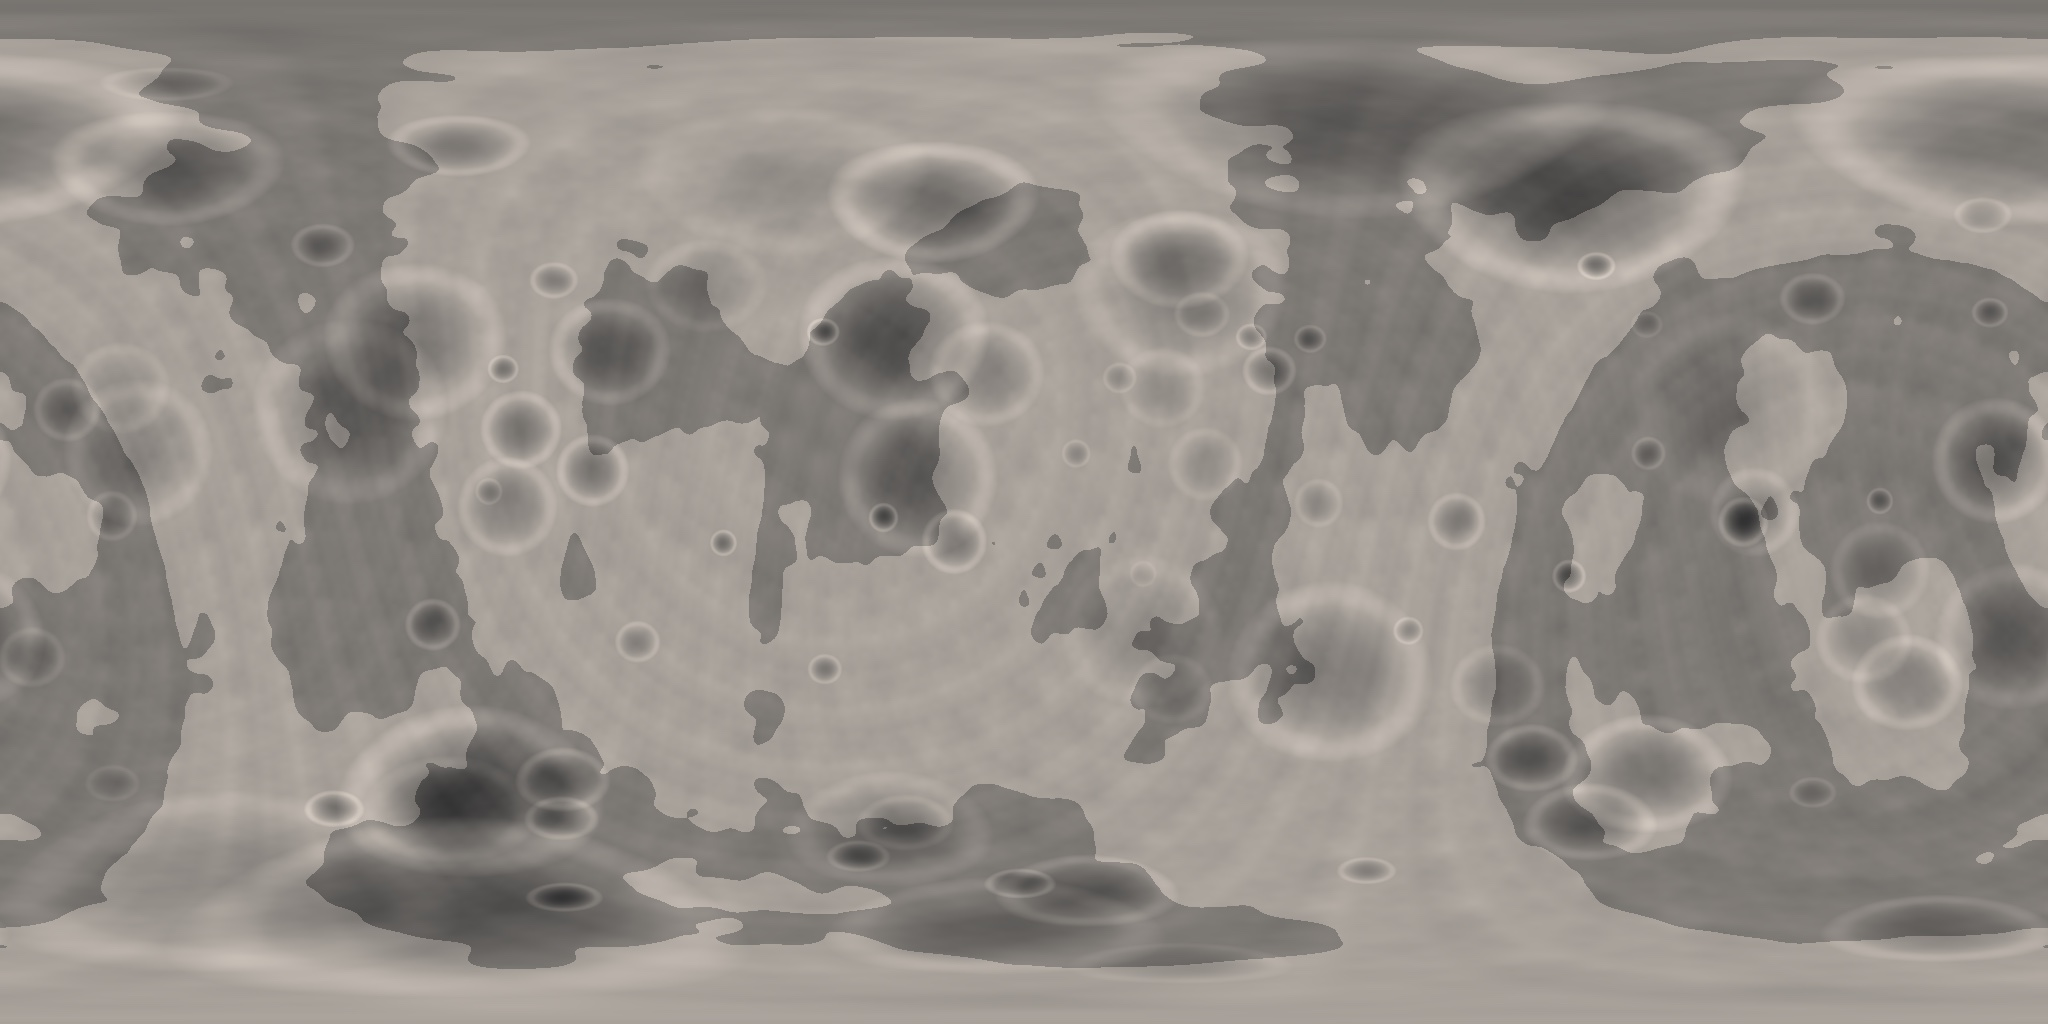
\includegraphics[width=\linewidth,height=4.4cm,keepaspectratio]{../public/textures/hd/vesta_dawn.jpg}\\[2pt]
{\scriptsize\itshape\color{orbitarMuted} Planiglob desfășurat: Harta topografică a protoplanetei 4 Vesta, obținută de sonda NASA Dawn în 2011--2012.}
\end{tabular}
\end{center}


\begin{tcolorbox}[orbitardata, title={\textbf{Repere esențiale: 4 Vesta}}]
\small
\begin{itemize}[leftmargin=1.4em, itemsep=2pt, topsep=2pt]
  \item \textbf{Clasificare și orbită:} Asteroid \quad$\bullet$\quad \textbf{Distanță:} 2,362 UA ($\approx$ 353 milioane de kilometri)
  \item \textbf{Dimensiuni și masă:} rază medie 262,7 de kilometri \quad$\bullet$\quad masă: 4,30e-5 $\times M_\oplus$
  \item \textbf{Gravitație și regim termic:} 0,025 $\times g_\oplus$ (0,25 m/s$^2$) \quad$\bullet$\quad temperatură medie: -60 $^\circ$C (înclinarea axei: Nespecificată)
  \item \textbf{Ciclu orbital și rotație:} perioadă orbitală (an): 1.325,75 zile ($\approx$ 3,63 ani pământești) \quad$\bullet$\quad rotație (zi): 5,34 ore (0,22 zile pământești) (elemente kepleriene: $a = 2,362$ UA, $e = 0,0890$, $i = 7,14^\circ$, $\Omega = 103,8^\circ$, $\omega = 151,2^\circ$)
  \item \textbf{Durata călătoriei de pe Pământ:} cu viteza luminii ($1c$): \emph{19 minute}; cu racheta ($50.000$ de kilometri pe oră): \emph{1,2 ani}; cu avionul ($900$ de kilometri pe oră): \emph{25 de ani}; cu mașina ($100$ de kilometri pe oră): \emph{230 de ani}.
  \item \textbf{Repere de scară și curiozitate:} Vesta este ca un cartof uriaș din stâncă, cu un munte la polul sud aproape la fel de înalt ca cel de pe Marte! Bucăți rupte din Vesta acum milioane de ani au căzut pe Pământ sub formă de meteoriți pe care îi putem vedea în muzee!
\end{itemize}
\end{tcolorbox}

\subsubsection*{Prezentare generală și profil astrofizic}
Descoperită în 1807 de Heinrich Olbers, 4 Vesta este o protoplanetă diferențiată (cu nucleu metalic, manta și scoarță bazaltică). Bazinul de impact Rheasilvia de la polul sud are 500 de kilometri diametru și un vârf central de 22 de kilometri înălțime. Vesta este un asteroid uriaș din piatră, atât de luminos încât uneori poate fi văzut de pe Pământ chiar și fără telescop, într-o noapte foarte senină! Vesta este ca un cartof uriaș din stâncă, cu un munte la polul sud aproape la fel de înalt ca cel de pe Marte!

\subsubsection*{Alcătuirea fizică și structura internă}
Privind în profunzimea sa, alcătuirea fizică este organizată pe mai multe straturi și regiuni distincte, fiecare având un rol bine definit în evoluția și dinamica acestui obiect cosmic. În primul rând se remarcă \textbf{Nucleu de fier-nichel (rază aproximativ 110 kilometri)}, dovadă că Vesta s-a topit și s-a diferențiat ca o planetă telurică în primele milioane de ani. În strânsă legătură cu această componentă se află \textbf{Manta de olivină}, expusă la suprafață în uriașul bazin de impact Rheasilvia. În completarea acestui ansamblu întâlnim \textbf{Scoarță bazaltică (sursa meteoriților HED)}, sursă pentru meteoriții de tip howardit-eucrit-diogenit găsiți pe Pământ.

\subsubsection*{Observații astronomice și istoricul explorării}
Orbitată și cartografiată în detaliu de sonda NASA Dawn între iulie 2011 și septembrie 2012. Bucăți rupte din Vesta acum milioane de ani au căzut pe Pământ sub formă de meteoriți pe care îi putem vedea în muzee!

\vspace{6pt}
\begin{tcolorbox}[orbitarquiz, title={\textbf{Întrebare de verificare \#38: 4 Vesta}}]
\textbf{Ce au descoperit oamenii de știință în centrul bazinului Rheasilvia de pe asteroidul Vesta?}
\begin{itemize}[leftmargin=2.2em, itemsep=2pt, topsep=4pt]
  \item[$\square$ \textbf{A.}] Un lac de apă
  \item[$\square$ \textbf{B.}] Un munte central înalt de 22 de kilometri, aproape cât Olympus Mons de pe Marte
  \item[$\square$ \textbf{C.}] Un vulcan activ
  \item[$\square$ \textbf{D.}] O sondă extraterestră
\end{itemize}
\vspace{2pt}
{\footnotesize\color{orbitarMuted}\textbf{Răspuns corect:} \textbf{B} (Un munte central înalt de 22 de kilometri, aproape cât Olympus Mons de pe Marte). \emph{Impactul colosal care a creat craterul Rheasilvia a ridicat în centru un munte de 22 de kilometri înălțime, unul dintre cele mai înalte vârfuri din Sistemul Solar.}}
\end{tcolorbox}
\clearpage


\subsection{2 Pallas}
\label{sec:body-pallas}
\vspace{-4pt}
{\large\itshape\color{orbitarAccent} Al doilea asteroid descoperit, cu o orbită puternic înclinată}\\[4pt]


\begin{center}
\begin{tabular}{@{}m{0.44\textwidth}@{\hspace{0.03\textwidth}}m{0.51\textwidth}@{}}
\centering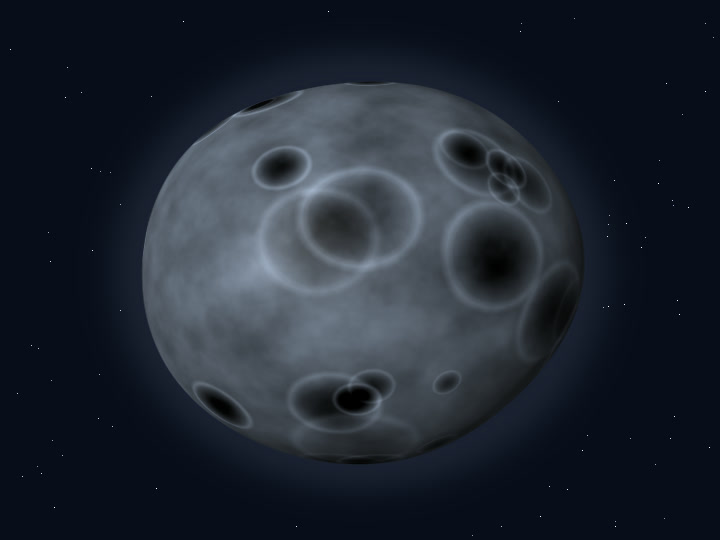
\includegraphics[width=\linewidth,height=4.4cm,keepaspectratio]{imagini/globuri/pallas.jpg}\\[2pt]
{\scriptsize\itshape\color{orbitarMuted} Vedere 3D a corpului ceresc (\textbf{2 Pallas})}
&
\centering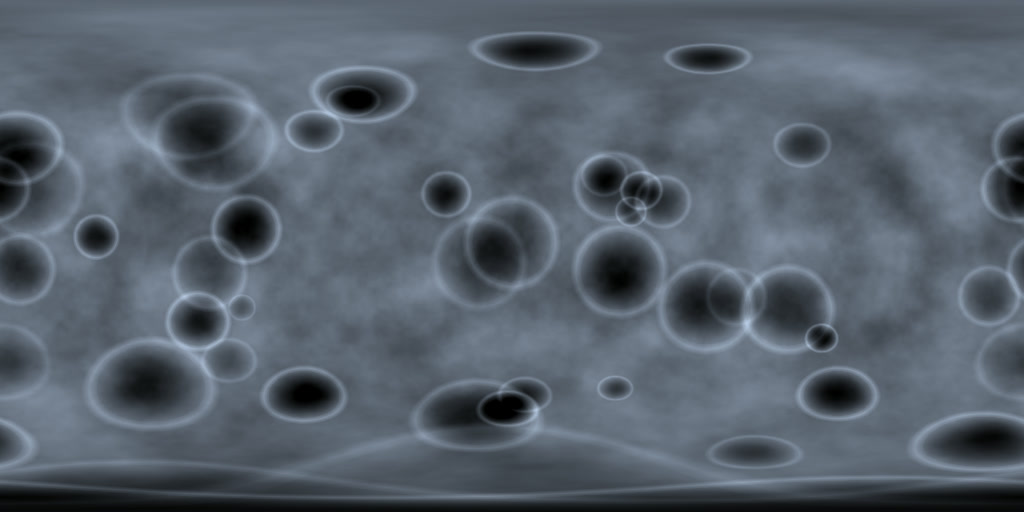
\includegraphics[width=\linewidth,height=4.4cm,keepaspectratio]{imagini/globuri/pallas_map.jpg}\\[2pt]
{\scriptsize\itshape\color{orbitarMuted} Planiglob desfășurat: Harta desfășurată a reliefului craterizat al asteroidului 2 Pallas din Centura Principală.}
\end{tabular}
\end{center}


\begin{tcolorbox}[orbitardata, title={\textbf{Repere esențiale: 2 Pallas}}]
\small
\begin{itemize}[leftmargin=1.4em, itemsep=2pt, topsep=2pt]
  \item \textbf{Clasificare și orbită:} Asteroid \quad$\bullet$\quad \textbf{Distanță:} 2,773 UA ($\approx$ 415 milioane de kilometri)
  \item \textbf{Dimensiuni și masă:} rază medie 256 de kilometri \quad$\bullet$\quad masă: 3,40e-5 $\times M_\oplus$
  \item \textbf{Gravitație și regim termic:} 0,022 $\times g_\oplus$ (0,22 m/s$^2$) \quad$\bullet$\quad temperatură medie: -109 $^\circ$C (înclinarea axei: Nespecificată)
  \item \textbf{Ciclu orbital și rotație:} perioadă orbitală (an): 1.685,9 zile ($\approx$ 4,62 ani pământești) \quad$\bullet$\quad rotație (zi): 7,81 ore (0,33 zile pământești) (elemente kepleriene: $a = 2,773$ UA, $e = 0,2310$, $i = 34,84^\circ$, $\Omega = 173,0^\circ$, $\omega = 310,0^\circ$)
  \item \textbf{Durata călătoriei de pe Pământ:} cu viteza luminii ($1c$): \emph{23 de minute}; cu racheta ($50.000$ de kilometri pe oră): \emph{2 ani}; cu avionul ($900$ de kilometri pe oră): \emph{33 de ani}; cu mașina ($100$ de kilometri pe oră): \emph{300 de ani}.
  \item \textbf{Repere de scară și curiozitate:} În timp ce majoritatea asteroizilor merg pe aceeași \guillemotleft{}autostradă\guillemotright{} în jurul Soarelui, Pallas zboară pe o pistă înclinată ca un montagne-russe! A fost al doilea asteroid descoperit vreodată, în anul 1802, la doar un an după Ceres!
\end{itemize}
\end{tcolorbox}

\subsubsection*{Prezentare generală și profil astrofizic}
Cu un diametru mediu de 512 kilometri, 2 Pallas conține aproximativ 7\% din masa Centurii de Asteroizi. Înclinarea orbitală neobișnuit de mare (34,8$^\circ$) provoacă coliziuni la viteze medii mult mai ridicate decât la alți asteroizi, dându-i o morfologie intens craterizată. Pallas este unul dintre cei mai mari asteroizi din Sistemul Solar și are o suprafață atât de plină de cratere încât seamănă cu o minge de golf! În timp ce majoritatea asteroizilor merg pe aceeași \guillemotleft{}autostradă\guillemotright{} în jurul Soarelui, Pallas zboară pe o pistă înclinată ca un montagne-russe!

\subsubsection*{Alcătuirea fizică și structura internă}
Privind în profunzimea sa, alcătuirea fizică este organizată pe mai multe straturi și regiuni distincte, fiecare având un rol bine definit în evoluția și dinamica acestui obiect cosmic. În primul rând se remarcă \textbf{Interior bogat în silicați hidratați}, compoziție asemănătoare condritelor carbonice sărace în apă. În strânsă legătură cu această componentă se află \textbf{Suprafață saturată de cratere (\guillemotleft{}golf-ball\guillemotright{})}, observată cu rezoluție înaltă prin instrumentul SPHERE al Very Large Telescope (ESO). În completarea acestui ansamblu întâlnim \textbf{Depozite luminoase de sare}, vizibile în unele cratere, indicând o evoluție termică timpurie.

\subsubsection*{Observații astronomice și istoricul explorării}
Descoperită în 1802 de Heinrich Olbers; din cauza înclinării orbitale mari (34,8$^\circ$), nicio sondă nu a putut încă să intre pe orbita sa. A fost al doilea asteroid descoperit vreodată, în anul 1802, la doar un an după Ceres!

\vspace{6pt}
\begin{tcolorbox}[orbitarquiz, title={\textbf{Întrebare de verificare \#39: 2 Pallas}}]
\textbf{De ce seamănă suprafața asteroidului Pallas cu o minge de golf?}
\begin{itemize}[leftmargin=2.2em, itemsep=2pt, topsep=4pt]
  \item[$\square$ \textbf{A.}] A fost sculptată de vânt
  \item[$\square$ \textbf{B.}] Orbita sa foarte înclinată (34,8$^\circ$) produce ciocniri extrem de violente și numeroase cu alți asteroizi
  \item[$\square$ \textbf{C.}] Este acoperită cu gheață moale
  \item[$\square$ \textbf{D.}] Are vulcani mici
\end{itemize}
\vspace{2pt}
{\footnotesize\color{orbitarMuted}\textbf{Răspuns corect:} \textbf{B} (Orbita sa foarte înclinată (34,8$^\circ$) produce ciocniri extrem de violente și numeroase cu alți asteroizi). \emph{Traversând centura de asteroizi sub un unghi mare, Pallas suferă impacturi la viteze de până la patru ori mai mari decât media din centură.}}
\end{tcolorbox}
\clearpage


\subsection{16 Psyche}
\label{sec:body-psyche}
\vspace{-4pt}
{\large\itshape\color{orbitarAccent} Lumea metalică unică din Centura de Asteroizi}\\[4pt]


\begin{center}
\begin{tabular}{@{}m{0.44\textwidth}@{\hspace{0.03\textwidth}}m{0.51\textwidth}@{}}
\centering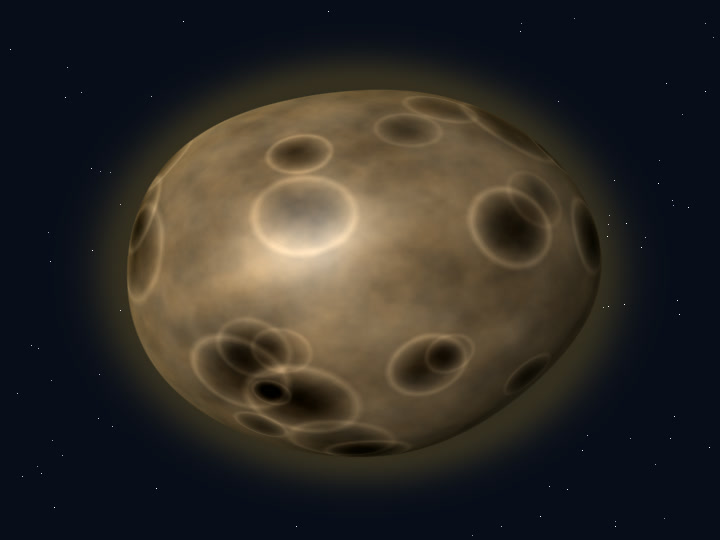
\includegraphics[width=\linewidth,height=4.4cm,keepaspectratio]{imagini/globuri/psyche.jpg}\\[2pt]
{\scriptsize\itshape\color{orbitarMuted} Vedere 3D a corpului ceresc (\textbf{16 Psyche})}
&
\centering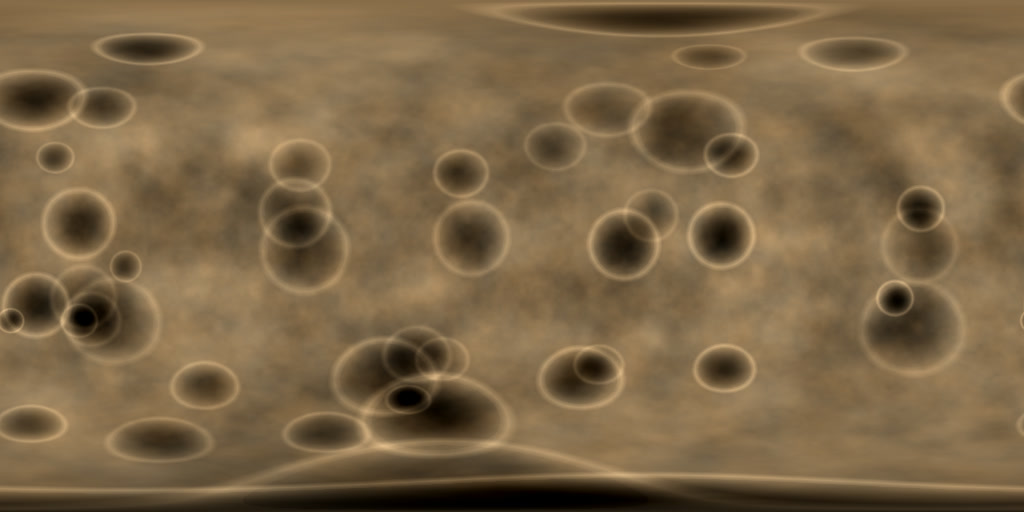
\includegraphics[width=\linewidth,height=4.4cm,keepaspectratio]{imagini/globuri/psyche_map.jpg}\\[2pt]
{\scriptsize\itshape\color{orbitarMuted} Planiglob desfășurat: Harta desfășurată a suprafeței bogate în fier și nichel a asteroidului metalic 16 Psyche.}
\end{tabular}
\end{center}


\begin{tcolorbox}[orbitardata, title={\textbf{Repere esențiale: 16 Psyche}}]
\small
\begin{itemize}[leftmargin=1.4em, itemsep=2pt, topsep=2pt]
  \item \textbf{Clasificare și orbită:} Asteroid \quad$\bullet$\quad \textbf{Distanță:} 2,923 UA ($\approx$ 437 milioane de kilometri)
  \item \textbf{Dimensiuni și masă:} rază medie 111 kilometri \quad$\bullet$\quad masă: 3,80e-6 $\times M_\oplus$
  \item \textbf{Gravitație și regim termic:} 0,015 $\times g_\oplus$ (0,15 m/s$^2$) \quad$\bullet$\quad temperatură medie: -100 $^\circ$C (înclinarea axei: Nespecificată)
  \item \textbf{Ciclu orbital și rotație:} perioadă orbitală (an): 1.823,9 zile ($\approx$ 4,99 ani pământești) \quad$\bullet$\quad rotație (zi): 4,20 ore (0,17 zile pământești) (elemente kepleriene: $a = 2,923$ UA, $e = 0,1340$, $i = 3,09^\circ$, $\Omega = 150,2^\circ$, $\omega = 227,5^\circ$)
  \item \textbf{Durata călătoriei de pe Pământ:} cu viteza luminii ($1c$): \emph{24 de minute}; cu racheta ($50.000$ de kilometri pe oră): \emph{5 ani și 10 luni (sonda Psyche)}; cu avionul ($900$ de kilometri pe oră): \emph{38 de ani}; cu mașina ($100$ de kilometri pe oră): \emph{340 de ani}.
  \item \textbf{Repere de scară și curiozitate:} Oamenii de știință cred că Psyche este inima de metal (nucleul) a unei planete străvechi care și-a pierdut învelișul de piatră! Deoarece nu putem săpa până în nucleul de fier al Pământului nostru, am trimis o sondă spațială să viziteze un nucleu planetar direct în spațiu, pe asteroidul Psyche!
\end{itemize}
\end{tcolorbox}

\subsubsection*{Prezentare generală și profil astrofizic}
Descoperit în 1852 de Annibale de Gasparis, 16 Psyche este cel mai masiv asteroid de tip M (metalic), având un diametru mediu de 222 de kilometri. Conține între 30\% și 60\% fier și nichel metalic amestecat cu silicați săraci în fier. Psyche este un asteroid cu totul special: în timp ce majoritatea asteroizilor sunt din piatră sau gheață, Psyche este făcut în mare parte din metal (fier și nichel)! Oamenii de știință cred că Psyche este inima de metal (nucleul) a unei planete străvechi care și-a pierdut învelișul de piatră!

\subsubsection*{Alcătuirea fizică și structura internă}
Privind în profunzimea sa, alcătuirea fizică este organizată pe mai multe straturi și regiuni distincte, fiecare având un rol bine definit în evoluția și dinamica acestui obiect cosmic. În primul rând se remarcă \textbf{Matrice metalică de fier-nichel}, posibil nucleul expus al unui planetesimal diferențiat timpuriu. În strânsă legătură cu această componentă se află \textbf{Cratere metalice și bazaltice}, două mari depresiuni de impact de aproximativ 90 de kilometri în emisfera sudică. În completarea acestui ansamblu întâlnim \textbf{Regolit mixt metal-silicat}, densitate medie de aproximativ 3,9--4,1 g/cm$^3$.

\subsubsection*{Observații astronomice și istoricul explorării}
Sonda NASA Psyche a fost lansată în octombrie 2023 cu propulsie electrică solară cu efect Hall și va intra pe orbita asteroidului în august 2029. Deoarece nu putem săpa până în nucleul de fier al Pământului nostru, am trimis o sondă spațială să viziteze un nucleu planetar direct în spațiu, pe asteroidul Psyche!

\vspace{6pt}
\begin{tcolorbox}[orbitarquiz, title={\textbf{Întrebare de verificare \#40: 16 Psyche}}]
\textbf{Din ce este alcătuit în proporție ridicată asteroidul 16 Psyche?}
\begin{itemize}[leftmargin=2.2em, itemsep=2pt, topsep=4pt]
  \item[$\square$ \textbf{A.}] Din gheață de metan
  \item[$\square$ \textbf{B.}] Din fier și nichel metalic (și silicați)
  \item[$\square$ \textbf{C.}] Din gaz hidrogen
  \item[$\square$ \textbf{D.}] Din apă lichidă
\end{itemize}
\vspace{2pt}
{\footnotesize\color{orbitarMuted}\textbf{Răspuns corect:} \textbf{B} (Din fier și nichel metalic (și silicați)). \emph{16 Psyche este cel mai mare asteroid de tip M, bogat în fier și nichel, oferind indicii despre cum s-au format nucleele planetelor telurice.}}
\end{tcolorbox}
\clearpage


\subsection{101955 Bennu}
\label{sec:body-bennu}
\vspace{-4pt}
{\large\itshape\color{orbitarAccent} Asteroid în formă de titirez din care NASA a adus mostre pe Pământ}\\[4pt]


\begin{center}
\begin{tabular}{@{}m{0.44\textwidth}@{\hspace{0.03\textwidth}}m{0.51\textwidth}@{}}
\centering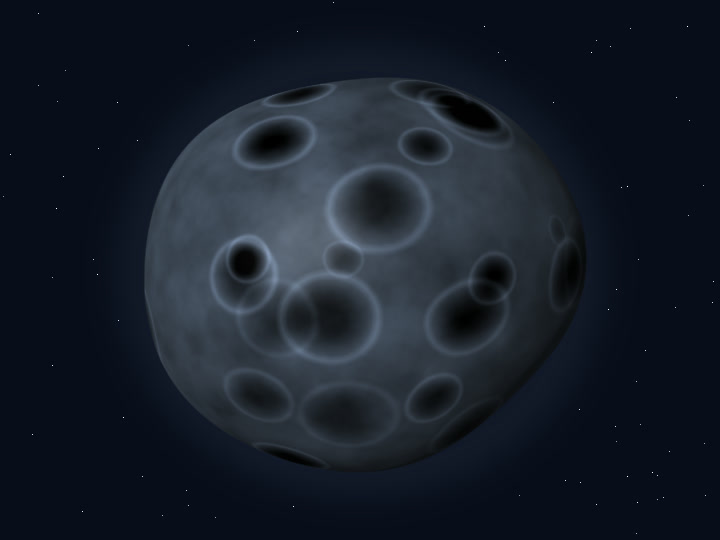
\includegraphics[width=\linewidth,height=4.4cm,keepaspectratio]{imagini/globuri/bennu.jpg}\\[2pt]
{\scriptsize\itshape\color{orbitarMuted} Vedere 3D a corpului ceresc (\textbf{101955 Bennu})}
&
\centering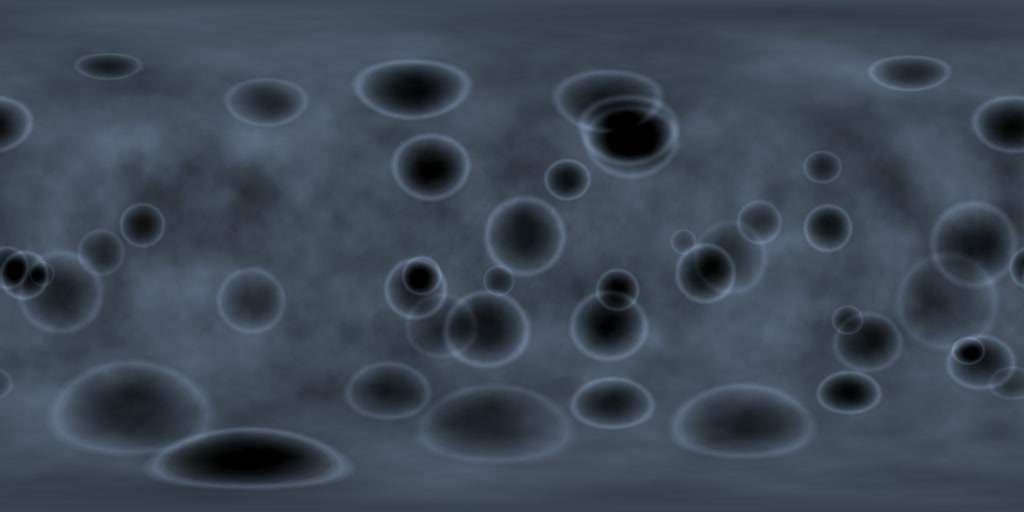
\includegraphics[width=\linewidth,height=4.4cm,keepaspectratio]{imagini/globuri/bennu_map.jpg}\\[2pt]
{\scriptsize\itshape\color{orbitarMuted} Planiglob desfășurat: Harta desfășurată a suprafeței carbonifere întunecate a asteroidului 101955 Bennu.}
\end{tabular}
\end{center}


\begin{tcolorbox}[orbitardata, title={\textbf{Repere esențiale: 101955 Bennu}}]
\small
\begin{itemize}[leftmargin=1.4em, itemsep=2pt, topsep=2pt]
  \item \textbf{Clasificare și orbită:} Asteroid \quad$\bullet$\quad \textbf{Distanță:} 1,126 UA ($\approx$ 168 milioane de kilometri)
  \item \textbf{Dimensiuni și masă:} rază medie 0,245 kilometri \quad$\bullet$\quad masă: 1,20e-11 $\times M_\oplus$
  \item \textbf{Gravitație și regim termic:} Microgravitație / Imponderabilitate ($\approx 0\,g$) \quad$\bullet$\quad temperatură medie: +4 $^\circ$C (înclinarea axei: Nespecificată)
  \item \textbf{Ciclu orbital și rotație:} perioadă orbitală (an): 436,65 zile ($\approx$ 1,20 ani pământești) \quad$\bullet$\quad rotație (zi): 4,30 ore (0,18 zile pământești) (elemente kepleriene: $a = 1,126$ UA, $e = 0,2040$, $i = 6,03^\circ$, $\Omega = 2,1^\circ$, $\omega = 66,2^\circ$)
  \item \textbf{Durata călătoriei de pe Pământ:} cu viteza luminii ($1c$): \emph{1,5 minute}; cu racheta ($50.000$ de kilometri pe oră): \emph{2 ani (OSIRIS-REx)}; cu avionul ($900$ de kilometri pe oră): \emph{3 ani și jumătate}; cu mașina ($100$ de kilometri pe oră): \emph{30 de ani (la apropiere)}.
  \item \textbf{Repere de scară și curiozitate:} Bennu este înalt cam cât o clădire zgârie-nori de 100 de etaje (aproximativ 500 de metri lățime)! Bennu nu este o piatră solidă, ci o grămadă de bolovani și pietriș ținuți împreună de o gravitație minusculă!
\end{itemize}
\end{tcolorbox}

\subsubsection*{Prezentare generală și profil astrofizic}
Asteroid apropiat de Pământ (grupul Apollo) de tip carbonic B, format prin agregarea gravitațională a fragmentelor (\guillemotleft{}rubble-pile\guillemotright{}). Este o capsulă a timpului chimică din primele 10 milioane de ani ale Sistemului Solar. Bennu este un mic asteroid în formă de titirez care trece pe lângă Pământ! O sondă spațială l-a atins și a adus acasă un pumn din pietricelele lui. Bennu este înalt cam cât o clădire zgârie-nori de 100 de etaje (aproximativ 500 de metri lățime)!

\subsubsection*{Alcătuirea fizică și structura internă}
Privind în profunzimea sa, alcătuirea fizică este organizată pe mai multe straturi și regiuni distincte, fiecare având un rol bine definit în evoluția și dinamica acestui obiect cosmic. În primul rând se remarcă \textbf{Structură internă tip \guillemotleft{}grămadă de moloz\guillemotright{} (Rubble Pile)}, cu 20--40\% spații goale în interior și o densitate de doar 1,19 g/cm$^3$. În strânsă legătură cu această componentă se află \textbf{Creastă ecuatorială pronunțată}, îi conferă forma de titirez sau diamant datorită rotației în 4,3 ore. În completarea acestui ansamblu întâlnim \textbf{Regolit bogat în carbon, apă legată în argile și fosfați}, unde 121,6 grame de eșantioane au fost aduse pe Pământ în septembrie 2023.

\subsubsection*{Observații astronomice și istoricul explorării}
Explorat de misiunea NASA OSIRIS-REx (2018--2021), care a colectat mostre din craterul Nightingale și le-a livrat pe Pământ în 2023. Bennu nu este o piatră solidă, ci o grămadă de bolovani și pietriș ținuți împreună de o gravitație minusculă!

\vspace{6pt}
\begin{tcolorbox}[orbitarquiz, title={\textbf{Întrebare de verificare \#41: 101955 Bennu}}]
\textbf{Ce misiune spațială a colectat mostre de pe asteroidul Bennu și le-a adus pe Pământ în 2023?}
\begin{itemize}[leftmargin=2.2em, itemsep=2pt, topsep=4pt]
  \item[$\square$ \textbf{A.}] Voyager 1
  \item[$\square$ \textbf{B.}] OSIRIS-REx
  \item[$\square$ \textbf{C.}] Cassini
  \item[$\square$ \textbf{D.}] Apollo 11
\end{itemize}
\vspace{2pt}
{\footnotesize\color{orbitarMuted}\textbf{Răspuns corect:} \textbf{B} (OSIRIS-REx). \emph{Sonda NASA OSIRIS-REx a colectat peste 120 de grame de regolit carbonic de pe Bennu și a parașutat capsula în deșertul Utah în septembrie 2023.}}
\end{tcolorbox}
\clearpage


\subsection{99942 Apophis}
\label{sec:body-apophis}
\vspace{-4pt}
{\large\itshape\color{orbitarAccent} Asteroidul care va trece în siguranță foarte aproape de Pământ în 2029}\\[4pt]


\begin{center}
\begin{tabular}{@{}m{0.44\textwidth}@{\hspace{0.03\textwidth}}m{0.51\textwidth}@{}}
\centering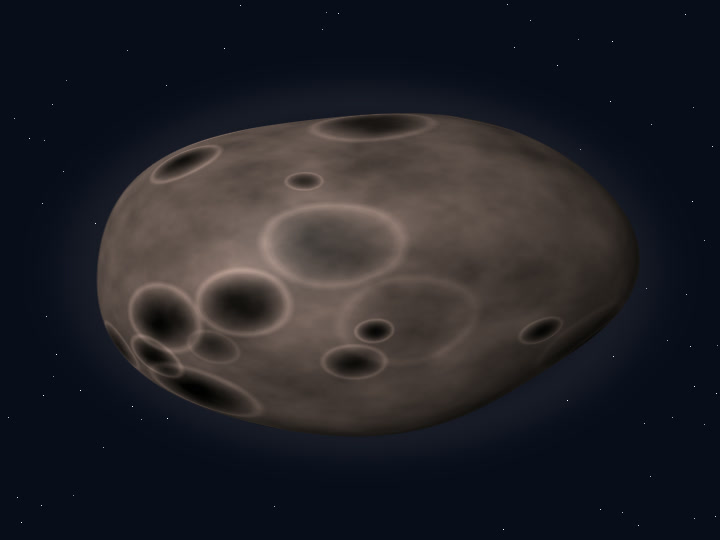
\includegraphics[width=\linewidth,height=4.4cm,keepaspectratio]{imagini/globuri/apophis.jpg}\\[2pt]
{\scriptsize\itshape\color{orbitarMuted} Vedere 3D a corpului ceresc (\textbf{99942 Apophis})}
&
\centering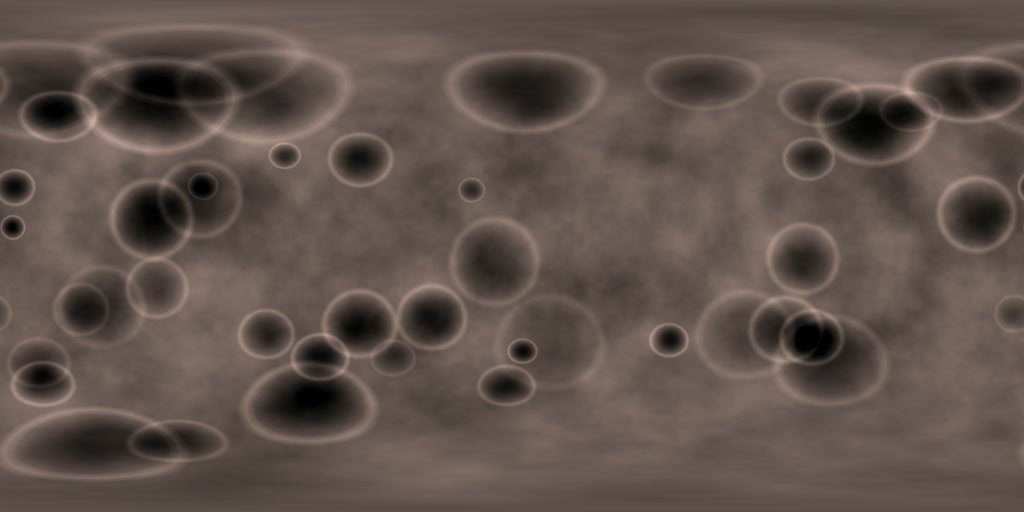
\includegraphics[width=\linewidth,height=4.4cm,keepaspectratio]{imagini/globuri/apophis_map.jpg}\\[2pt]
{\scriptsize\itshape\color{orbitarMuted} Planiglob desfășurat: Harta desfășurată a suprafeței stâncoase a asteroidului din apropierea Pământului 99942 Apophis.}
\end{tabular}
\end{center}


\begin{tcolorbox}[orbitardata, title={\textbf{Repere esențiale: 99942 Apophis}}]
\small
\begin{itemize}[leftmargin=1.4em, itemsep=2pt, topsep=2pt]
  \item \textbf{Clasificare și orbită:} Asteroid \quad$\bullet$\quad \textbf{Distanță:} 0,922 UA ($\approx$ 138 milioane de kilometri)
  \item \textbf{Dimensiuni și masă:} rază medie 0,185 kilometri \quad$\bullet$\quad masă: 4,00e-12 $\times M_\oplus$
  \item \textbf{Gravitație și regim termic:} Microgravitație / Imponderabilitate ($\approx 0\,g$) \quad$\bullet$\quad temperatură medie: +17 $^\circ$C (înclinarea axei: Nespecificată)
  \item \textbf{Ciclu orbital și rotație:} perioadă orbitală (an): 323,6 zile pământești \quad$\bullet$\quad rotație (zi): 30,56 ore (1,27 zile pământești) (elemente kepleriene: $a = 0,922$ UA, $e = 0,1910$, $i = 3,34^\circ$, $\Omega = 204,4^\circ$, $\omega = 126,4^\circ$)
  \item \textbf{Durata călătoriei de pe Pământ:} cu viteza luminii ($1c$): \emph{0,1 secunde la perigeul din 2029}; cu racheta ($50.000$ de kilometri pe oră): \emph{câteva luni pe o traiectorie de întâlnire}; cu avionul ($900$ de kilometri pe oră): \emph{36 de ore (în 2029)}; cu mașina ($100$ de kilometri pe oră): \emph{13 zile la apropierea din 2029}.
  \item \textbf{Repere de scară și curiozitate:} Apophis are mărimea a trei terenuri de fotbal puse cap la cap (aproximativ 370 de metri)! Pe 13 aprilie 2029, Apophis va trece în deplină siguranță la doar 32.000 de kilometri de Pământ, adică mai aproape decât unii sateliți de televiziune!
\end{itemize}
\end{tcolorbox}

\subsubsection*{Prezentare generală și profil astrofizic}
Asteroid de tip S (silicatic) din grupul Aten. Măsurătorile radar de înaltă precizie au confirmat că nu există niciun risc de impact cu Pământul pentru cel puțin următoarea sută de ani, dar survolul din 13 aprilie 2029 va fi o oportunitate științifică unică. Apophis este un asteroid în formă de arahidă care în anul 2029 ne va face o vizită pașnică, trecând pe cer ca o steluță vizibilă cu ochiul liber! Apophis are mărimea a trei terenuri de fotbal puse cap la cap (aproximativ 370 de metri)!

\subsubsection*{Alcătuirea fizică și structura internă}
Privind în profunzimea sa, alcătuirea fizică este organizată pe mai multe straturi și regiuni distincte, fiecare având un rol bine definit în evoluția și dinamica acestui obiect cosmic. În primul rând se remarcă \textbf{Formă bilobată (de arahidă)}, determinată prin imagistică radar de la observatorul Goldstone. În strânsă legătură cu această componentă se află \textbf{Compoziție de condrite ordinare, fier și nichel}, tipică asteroizilor stâncoși de clasă Sq. În completarea acestui ansamblu întâlnim \textbf{Rotație complexă (tumbling)}, unde forțele mareice terestre din 2029 îi vor modifica ușor rotația și orbita.

\subsubsection*{Observații astronomice și istoricul explorării}
Va fi studiat de aproape în 2029 de sonda NASA OSIRIS-APEX (fosta OSIRIS-REx) și de misiunea europeană RAMSES (ESA). Pe 13 aprilie 2029, Apophis va trece în deplină siguranță la doar 32.000 de kilometri de Pământ, adică mai aproape decât unii sateliți de televiziune!

\vspace{6pt}
\begin{tcolorbox}[orbitarquiz, title={\textbf{Întrebare de verificare \#42: 99942 Apophis}}]
\textbf{Ce se va întâmpla pe 13 aprilie 2029 cu asteroidul Apophis?}
\begin{itemize}[leftmargin=2.2em, itemsep=2pt, topsep=4pt]
  \item[$\square$ \textbf{A.}] Va intra pe orbita lui Jupiter
  \item[$\square$ \textbf{B.}] Va trece în deplină siguranță la aproximativ 32.000 de kilometri de Pământ, fiind vizibil cu ochiul liber
  \item[$\square$ \textbf{C.}] Se va topi lângă Soare
  \item[$\square$ \textbf{D.}] Va lovi Luna
\end{itemize}
\vspace{2pt}
{\footnotesize\color{orbitarMuted}\textbf{Răspuns corect:} \textbf{B} (Va trece în deplină siguranță la aproximativ 32.000 de kilometri de Pământ, fiind vizibil cu ochiul liber). \emph{Calculele radar au demonstrat că Apophis va trece fără niciun pericol la aproximativ 32.000 de kilometri de Pământ, oferind astronomilor ocazia rară de a-l studia de aproape.}}
\end{tcolorbox}
\clearpage

